\section{Results}

\Cref{fig:dem_ts_aug_04_2011}, \cref{fig:dem_ts_aug_31_2012} and \cref{fig:dem_ts_oct_28_2021} shows the timeseries plot of DEM for the three events. The time series plot is calculated by averaging the acceptable DEM solutions obtained for each image over three consecutive temperature range (i.e averaging the solutions for 5.85, 5.9 and 5.95 etc.). Blue curve corresponds to the full disk DEM and red curve corresponds to the point source DEM. The temperature range above logT=6.75 has been omitted as no correlation was found between point source and full disk.

\begin{figure}[h!]
    \centering
    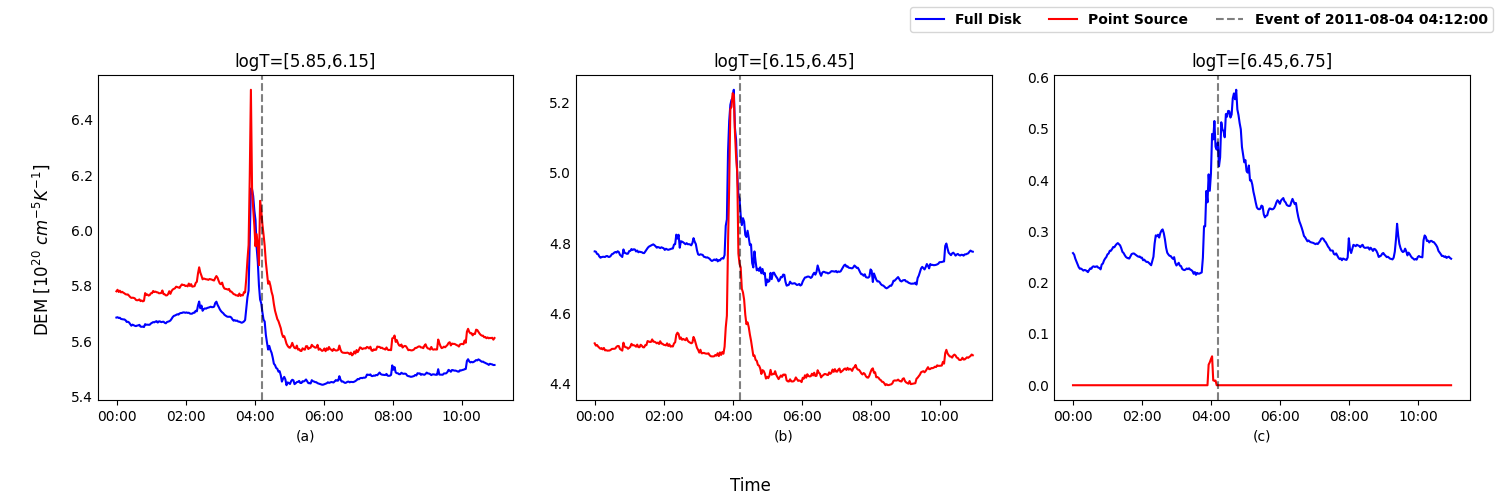
\includegraphics[width=\textwidth]{images/dem_ts_aug_04_2011.png}
    \caption[DEM Timeseries for \nth{4} August 2011 Event]{Timeseries of DEM for \nth{4} August 2011 Event.}
    \label{fig:dem_ts_aug_04_2011}
\end{figure}

\begin{figure}[h!]
    \centering
    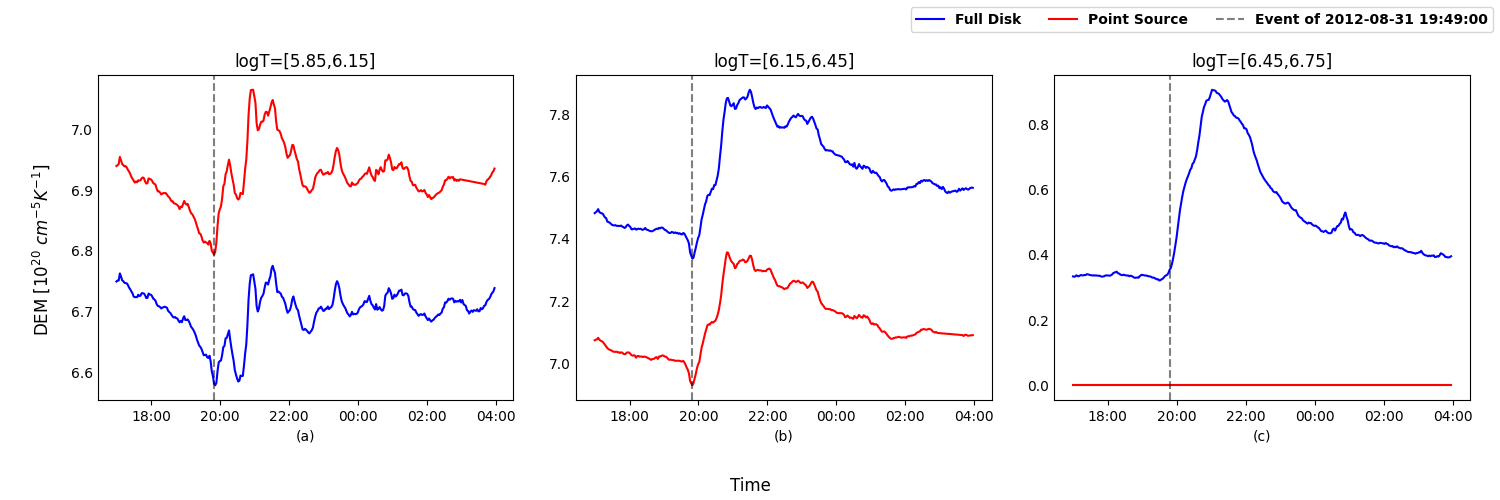
\includegraphics[width=\textwidth]{images/dem_ts_aug_31_2012.png}
    \caption[DEM Timeseries for \nth{31} August 2012 Event]{Timeseries of DEM for \nth{31} August 2012 Event}
    \label{fig:dem_ts_aug_31_2012}
\end{figure}

\begin{figure}[h!]
    \centering
    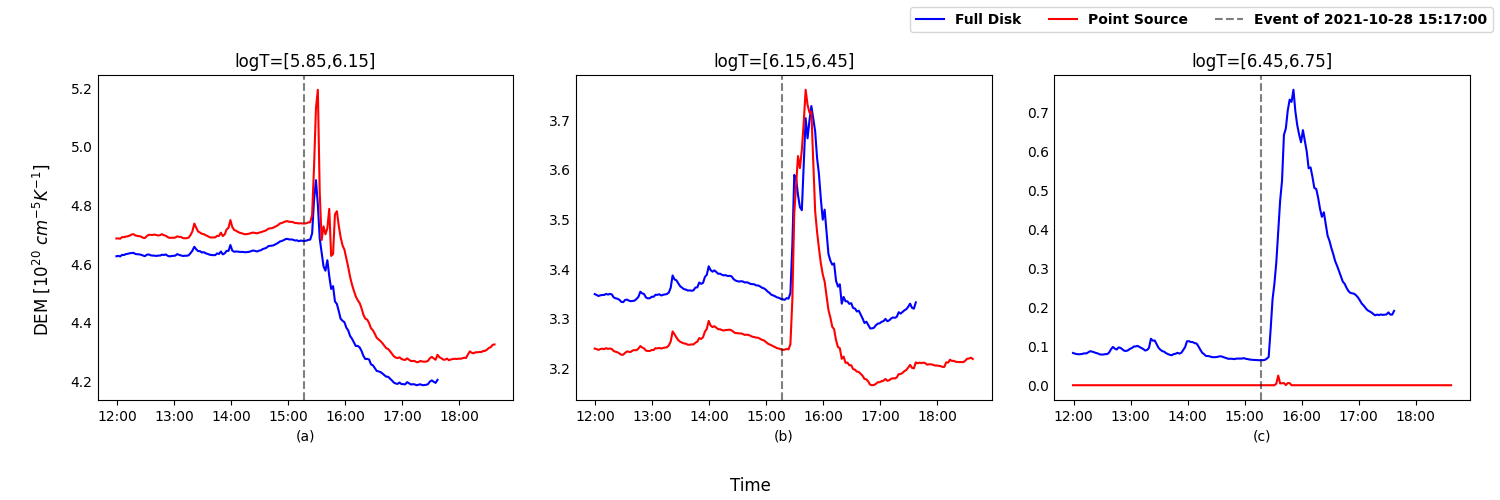
\includegraphics[width=\textwidth]{images/dem_ts_oct_28_2021.png}
    \caption[DEM Timeseries for \nth{28} October 2021 Event]{Timeseries of DEM for \nth{28} October 2021 Event}
    \label{fig:dem_ts_oct_28_2021}
\end{figure}

In \cref{fig:dem_ts_aug_04_2011}(a) and \cref{fig:dem_ts_aug_04_2011}(b), we can observe the coronal dimming or decrease in the DEM value after the event spike. But, in \cref{fig:dem_ts_aug_04_2011}(c) no dimming is observed. Dimming is the most prominent in logT = [5.85, 6.15]. This means that the mass loss of coronal plasma is mostly seen in this temperature range. The sudden increase in the DEM curve is due to the solar flare which is associated with the CME. There is very high correlation for the first two temperature ranges, but there is little to no correlation in the DEM profiles of the full disk and point source for the temperature range logT=[6.45, 6.75]. For temperature ranges greater than logT=6.45, the correlation is almost 0. We make use of Pearson's Correlation coeffecient (\cref{eqn:pearsonr}) to find out the amount of correlation between the point source and full disk DEM, for which we use \texttt{pearsonr} function from the \texttt{scipy} library in Python. The pearson correlation coeffecient r between two datasets \textbf{x} and \textbf{y} is calculated using the formula,

\begin{equation}
    \label{eqn:pearsonr}
    r = \frac{\sum (x_i - \overline{x})(y_i - \overline{y})}{\sqrt{\sum (x_i - \overline{x})^2 \sum (y_i - \overline{y})^2}}
\end{equation}\hspace{0.25cm}

\begin{table}[h!]
    \centering
    \begin{tblr}{
          cell{1}{1} = {r=2}{},
          cell{1}{2} = {c=3}{c},
          vline{1-5} = {-}{},
          hline{1-6} = {-}{},
        }
        \textbf{Event} & \textbf{Pearson Correlation Coeffecient} &         & \\
        & logT=[5.85, 6.15]  & logT=[6.15, 6.45] & logT=[6.45, 6.75] \\
        \nth{4} August 2011  & 0.9449 & 0.9767 & 0.2190\\
        \nth{31} August 2012  & 0.7027 & 0.9885 & 0.2079\\
        \nth{28} October 2021 & 0.9555 & 0.9577 & 0.2578 \\
    \end{tblr}
    \caption{Correlation between Point source and Full Disk DEM}
\end{table}

The correlation in the DEM curves of the point source and full disk below logT $\le$ 6.45 means that point source image of Sun shows characteristic behaviours like coronal dimming associated with the CMEs, filament eruption associated CMEs and GLE CME signatures seen in the case of full disk image of Sun.\\

\label{para:dem_discrepancy}
We see a discrepancy in the value of DEM between the point source and full disk average values. This could be due to the error induced during the DEM profile reconstruction, instrumental and averaging error. As seen in \cref{fig:dem_img_aug_4_2011}, the noise pixels in the corners of the image, due to the diffraction of light with the AIA telescopes, affect the pointification process, inducing high errors. The dataset length is not equal in some of the case as invalid or small DEM solution values have been removed.\\

\begin{figure}[h!]

    \begin{subfigure}[b]{0.3\textwidth}
        \centering
        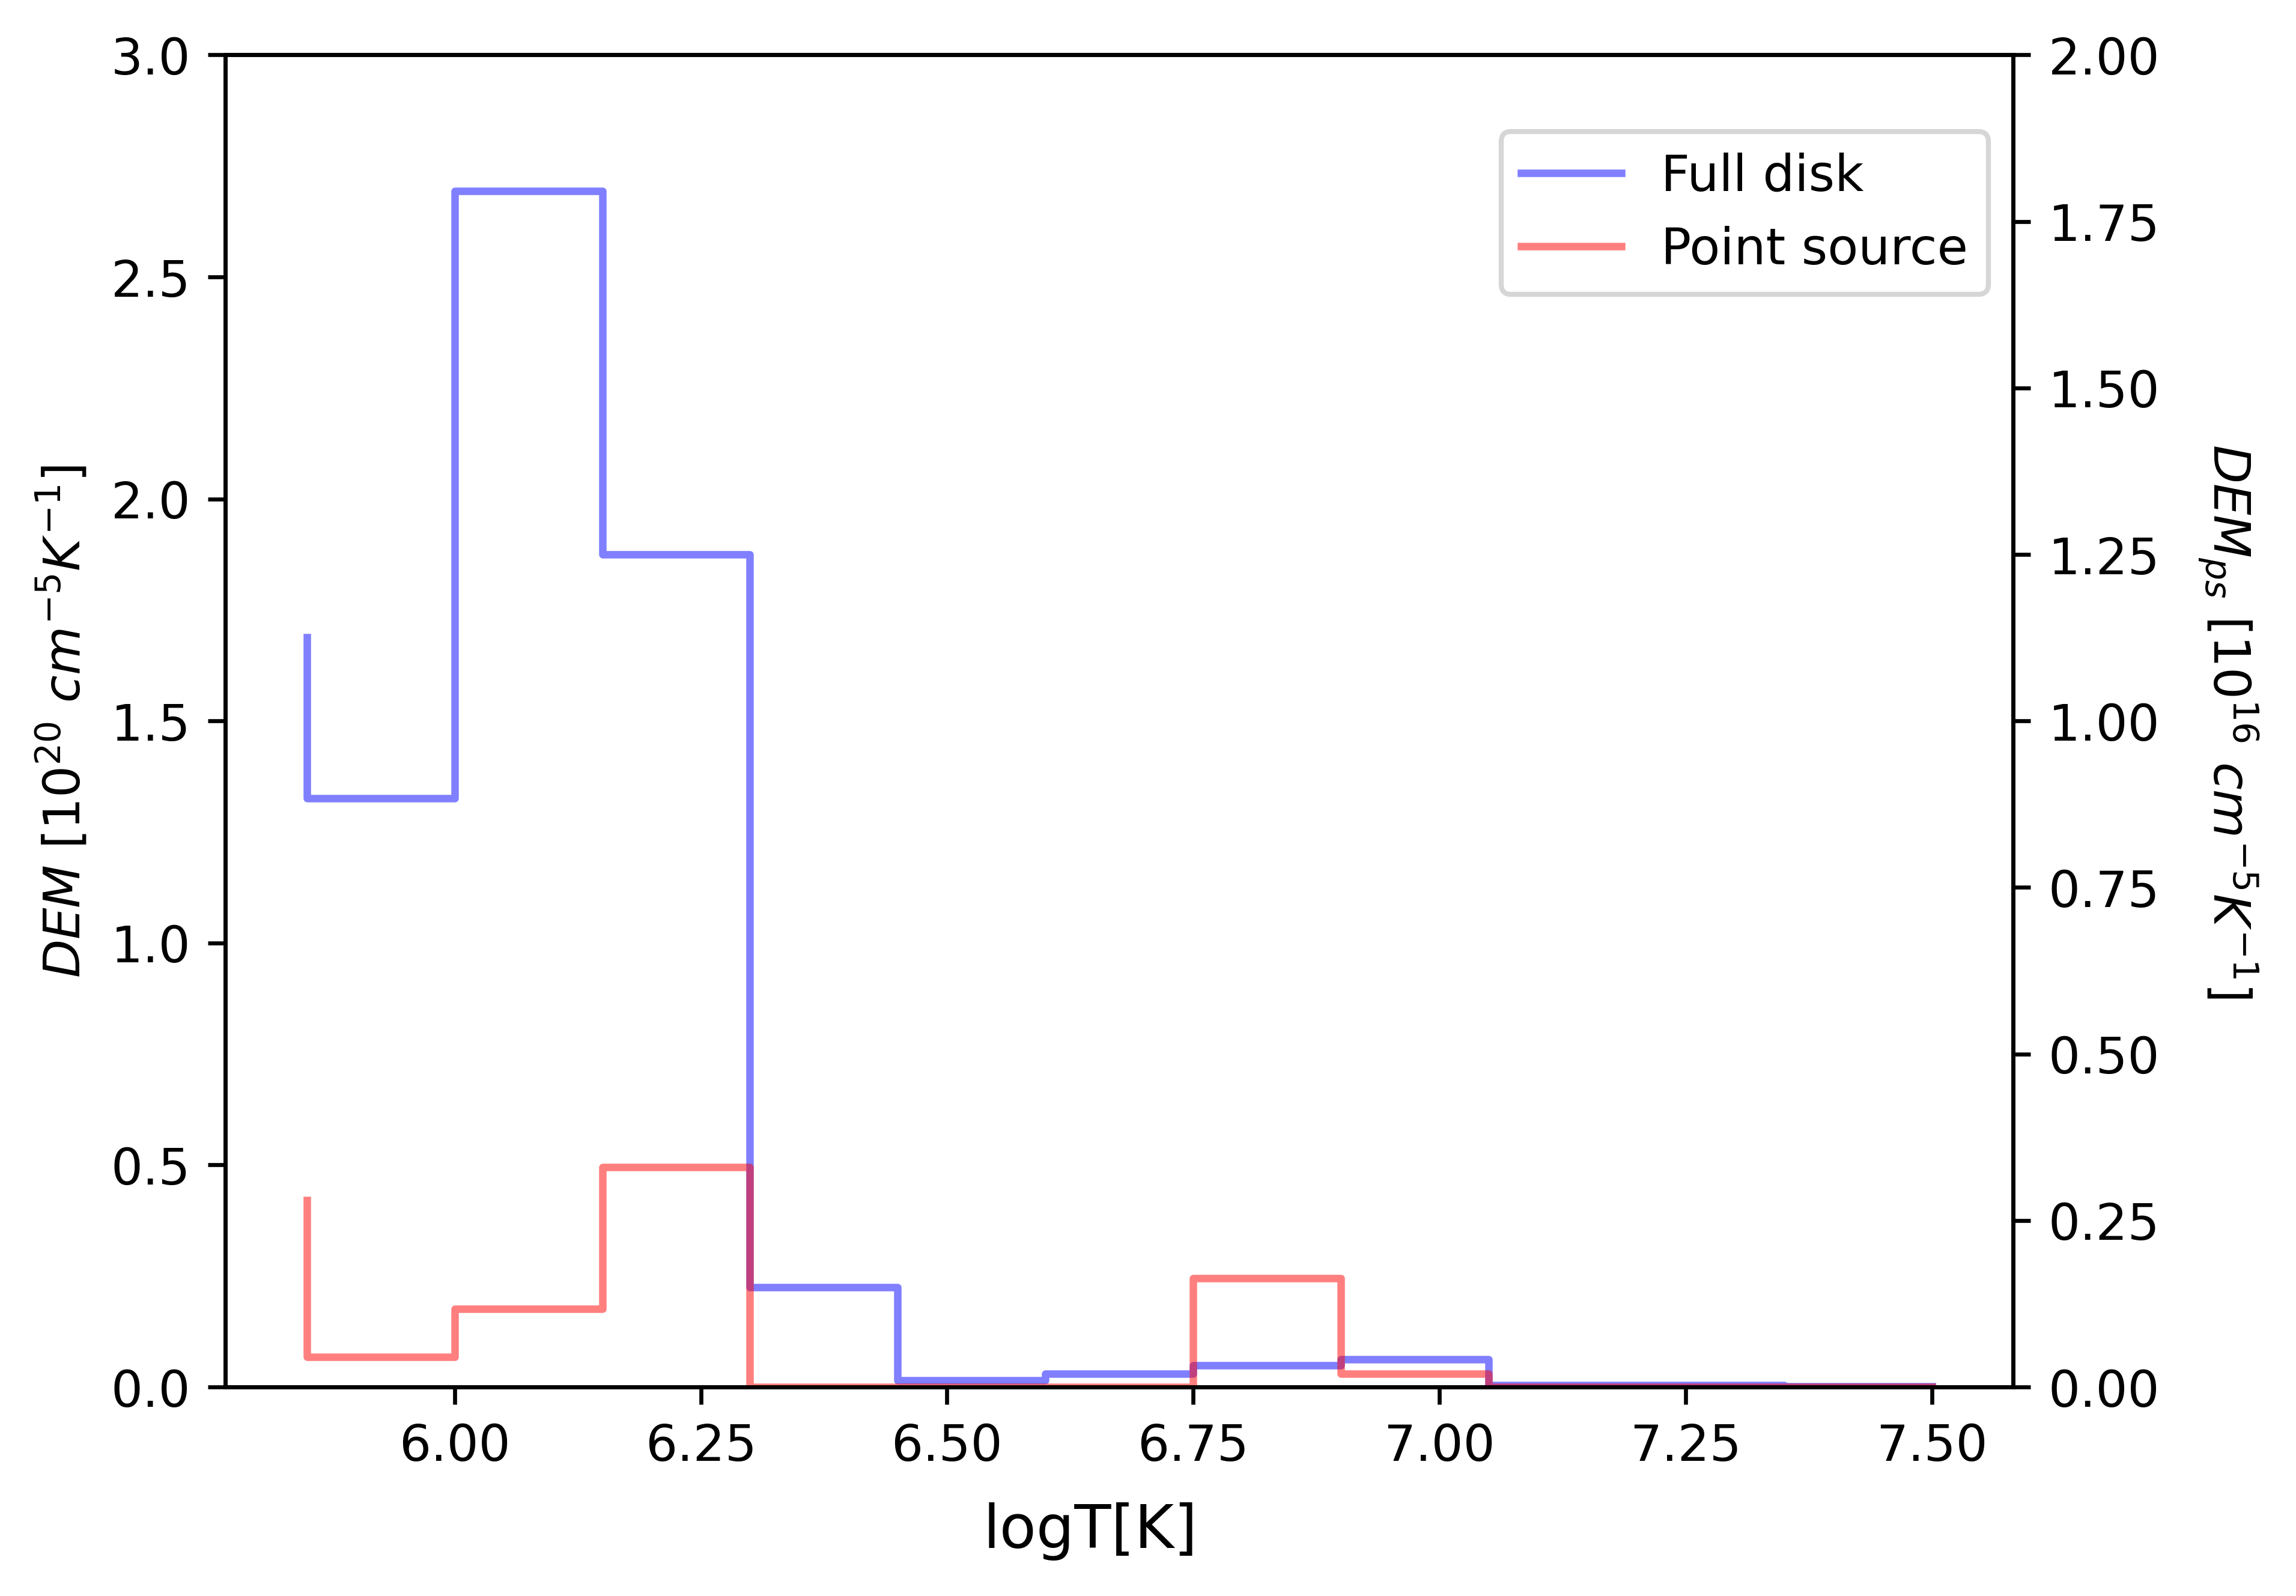
\includegraphics[width=\textwidth]{images/dem_profile_before_event_2011_aug_04.png}
        \caption{Before event (02:21 UT)}
    \end{subfigure}
    \hfill
    \begin{subfigure}[b]{0.3\textwidth}
        \centering
        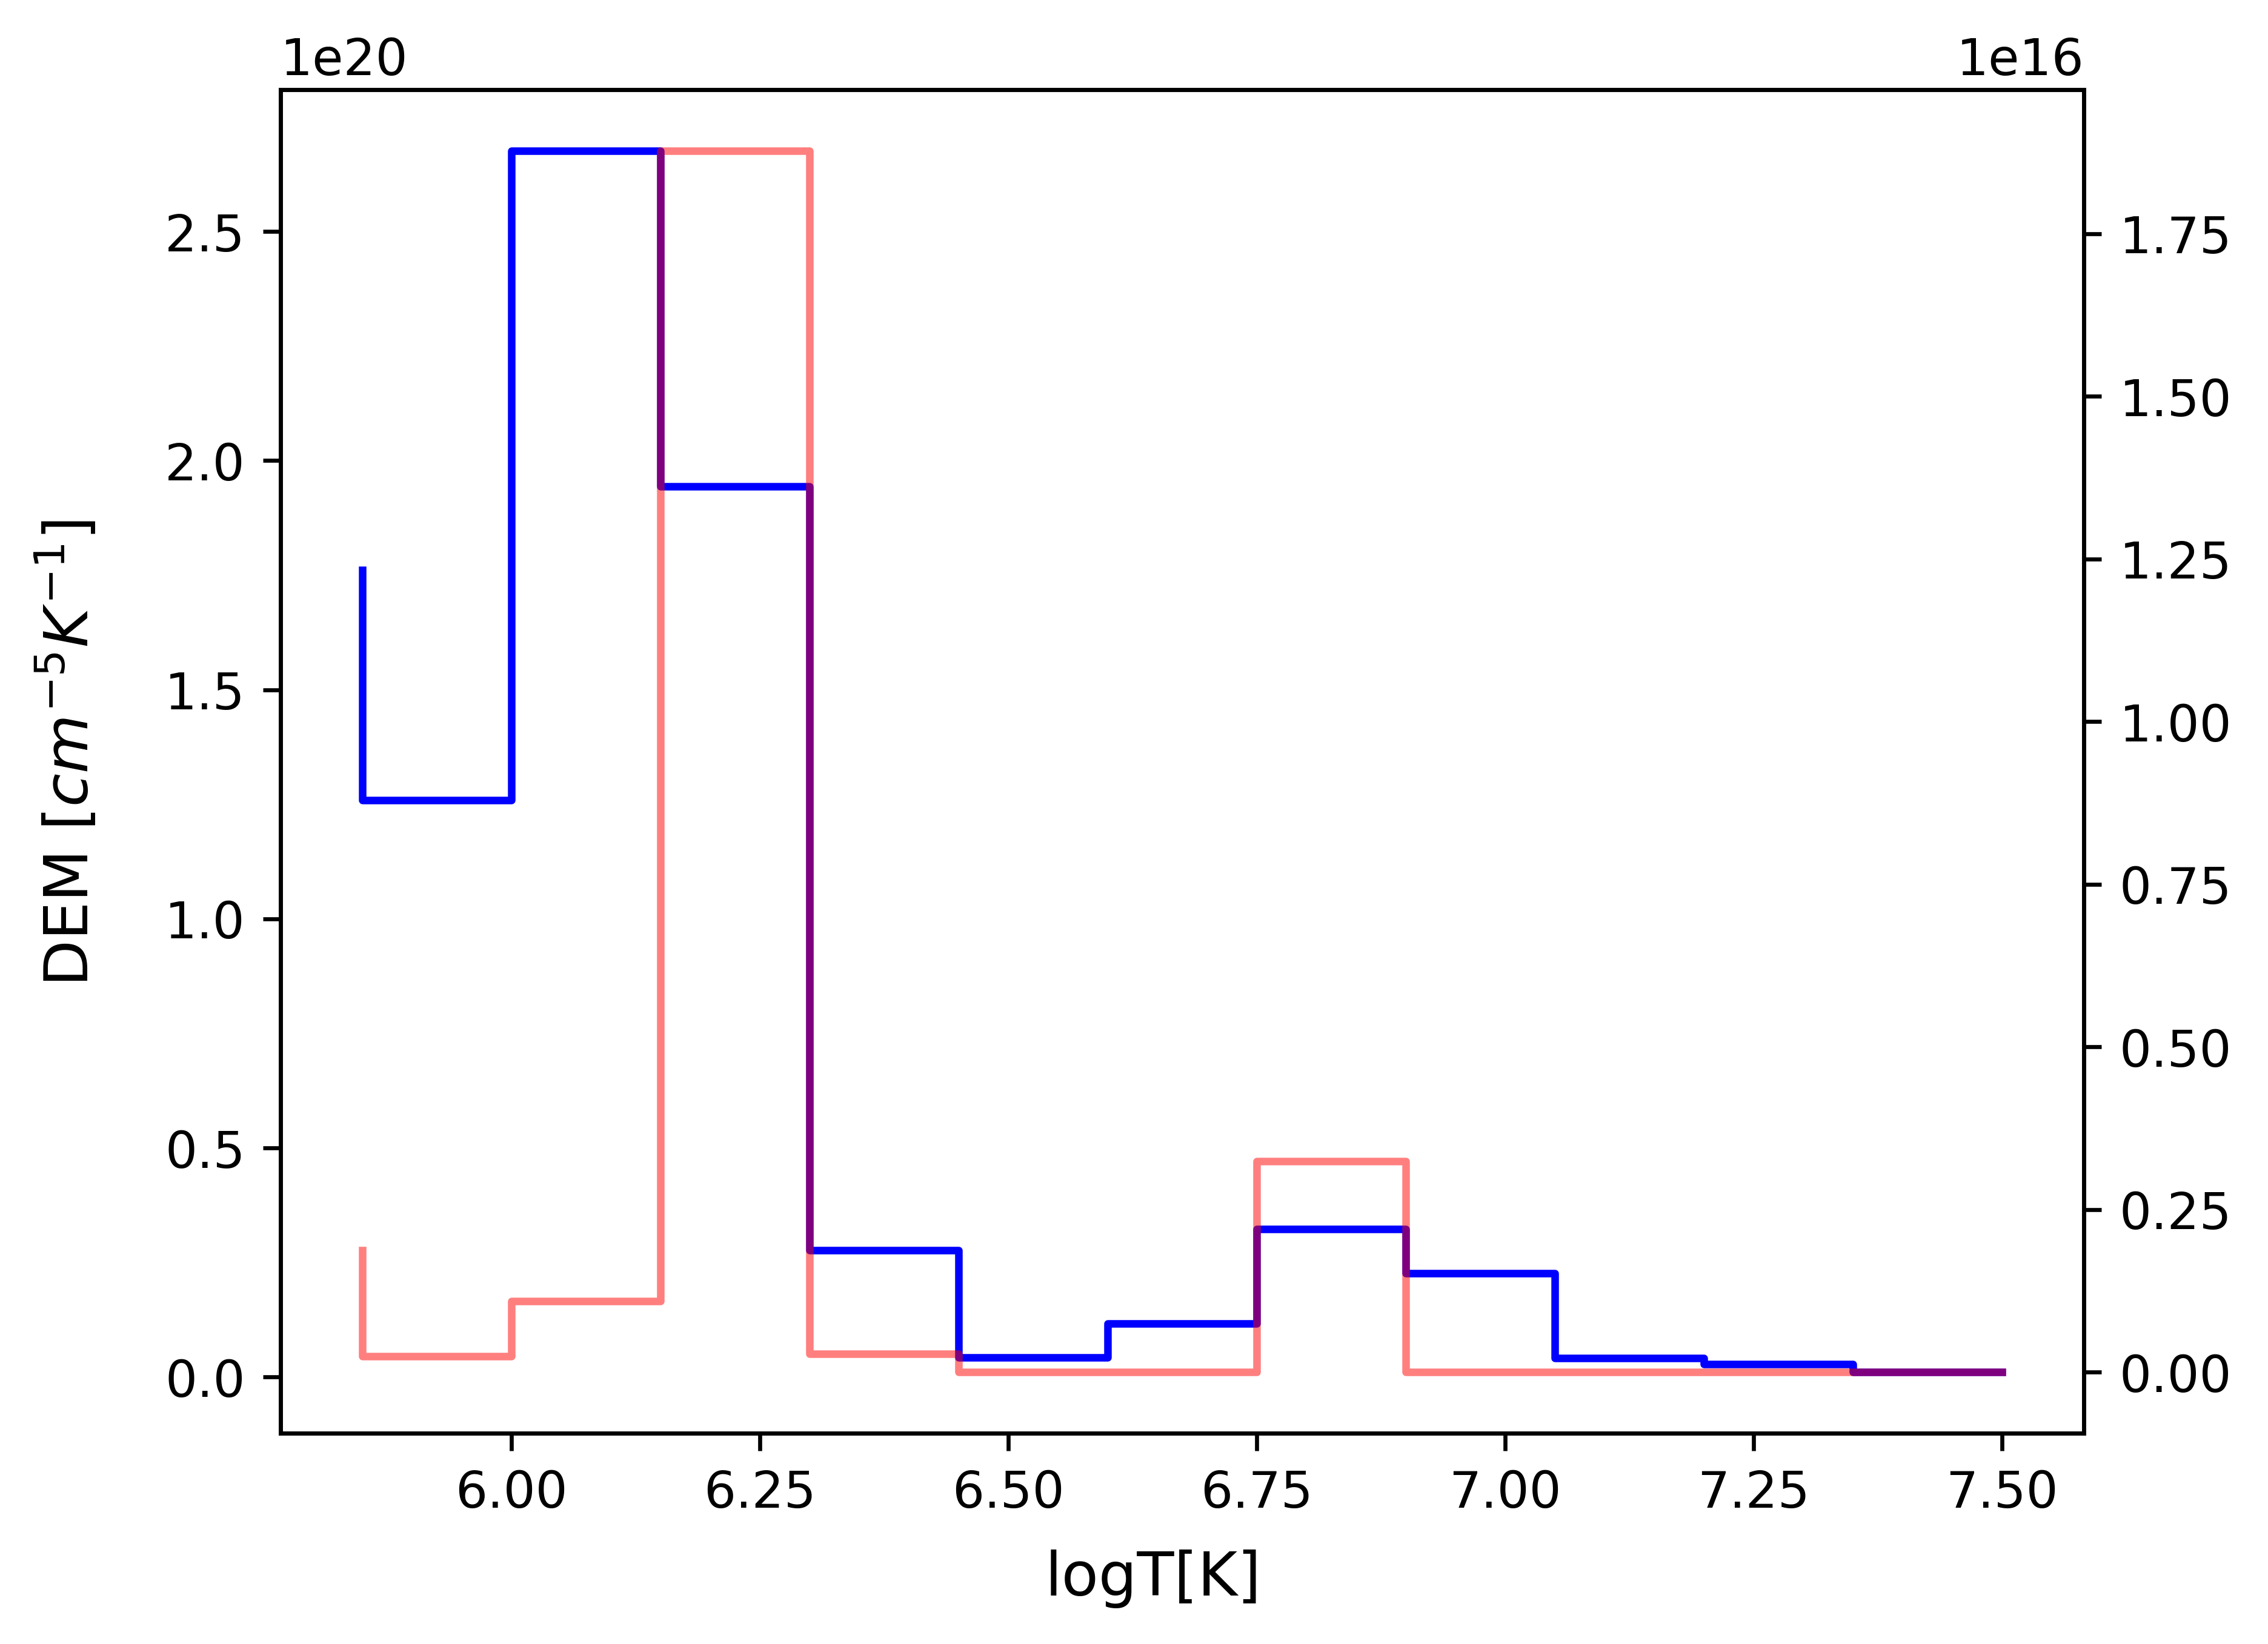
\includegraphics[width=\textwidth]{images/dem_profile_during_event_2011_aug_04.png}
        \caption{During event (04:11 UT)}
        \label{fig:dem_pro_aug_04_2011_b}
    \end{subfigure}
    \hfill
    \begin{subfigure}[b]{0.3\textwidth}
        \centering
        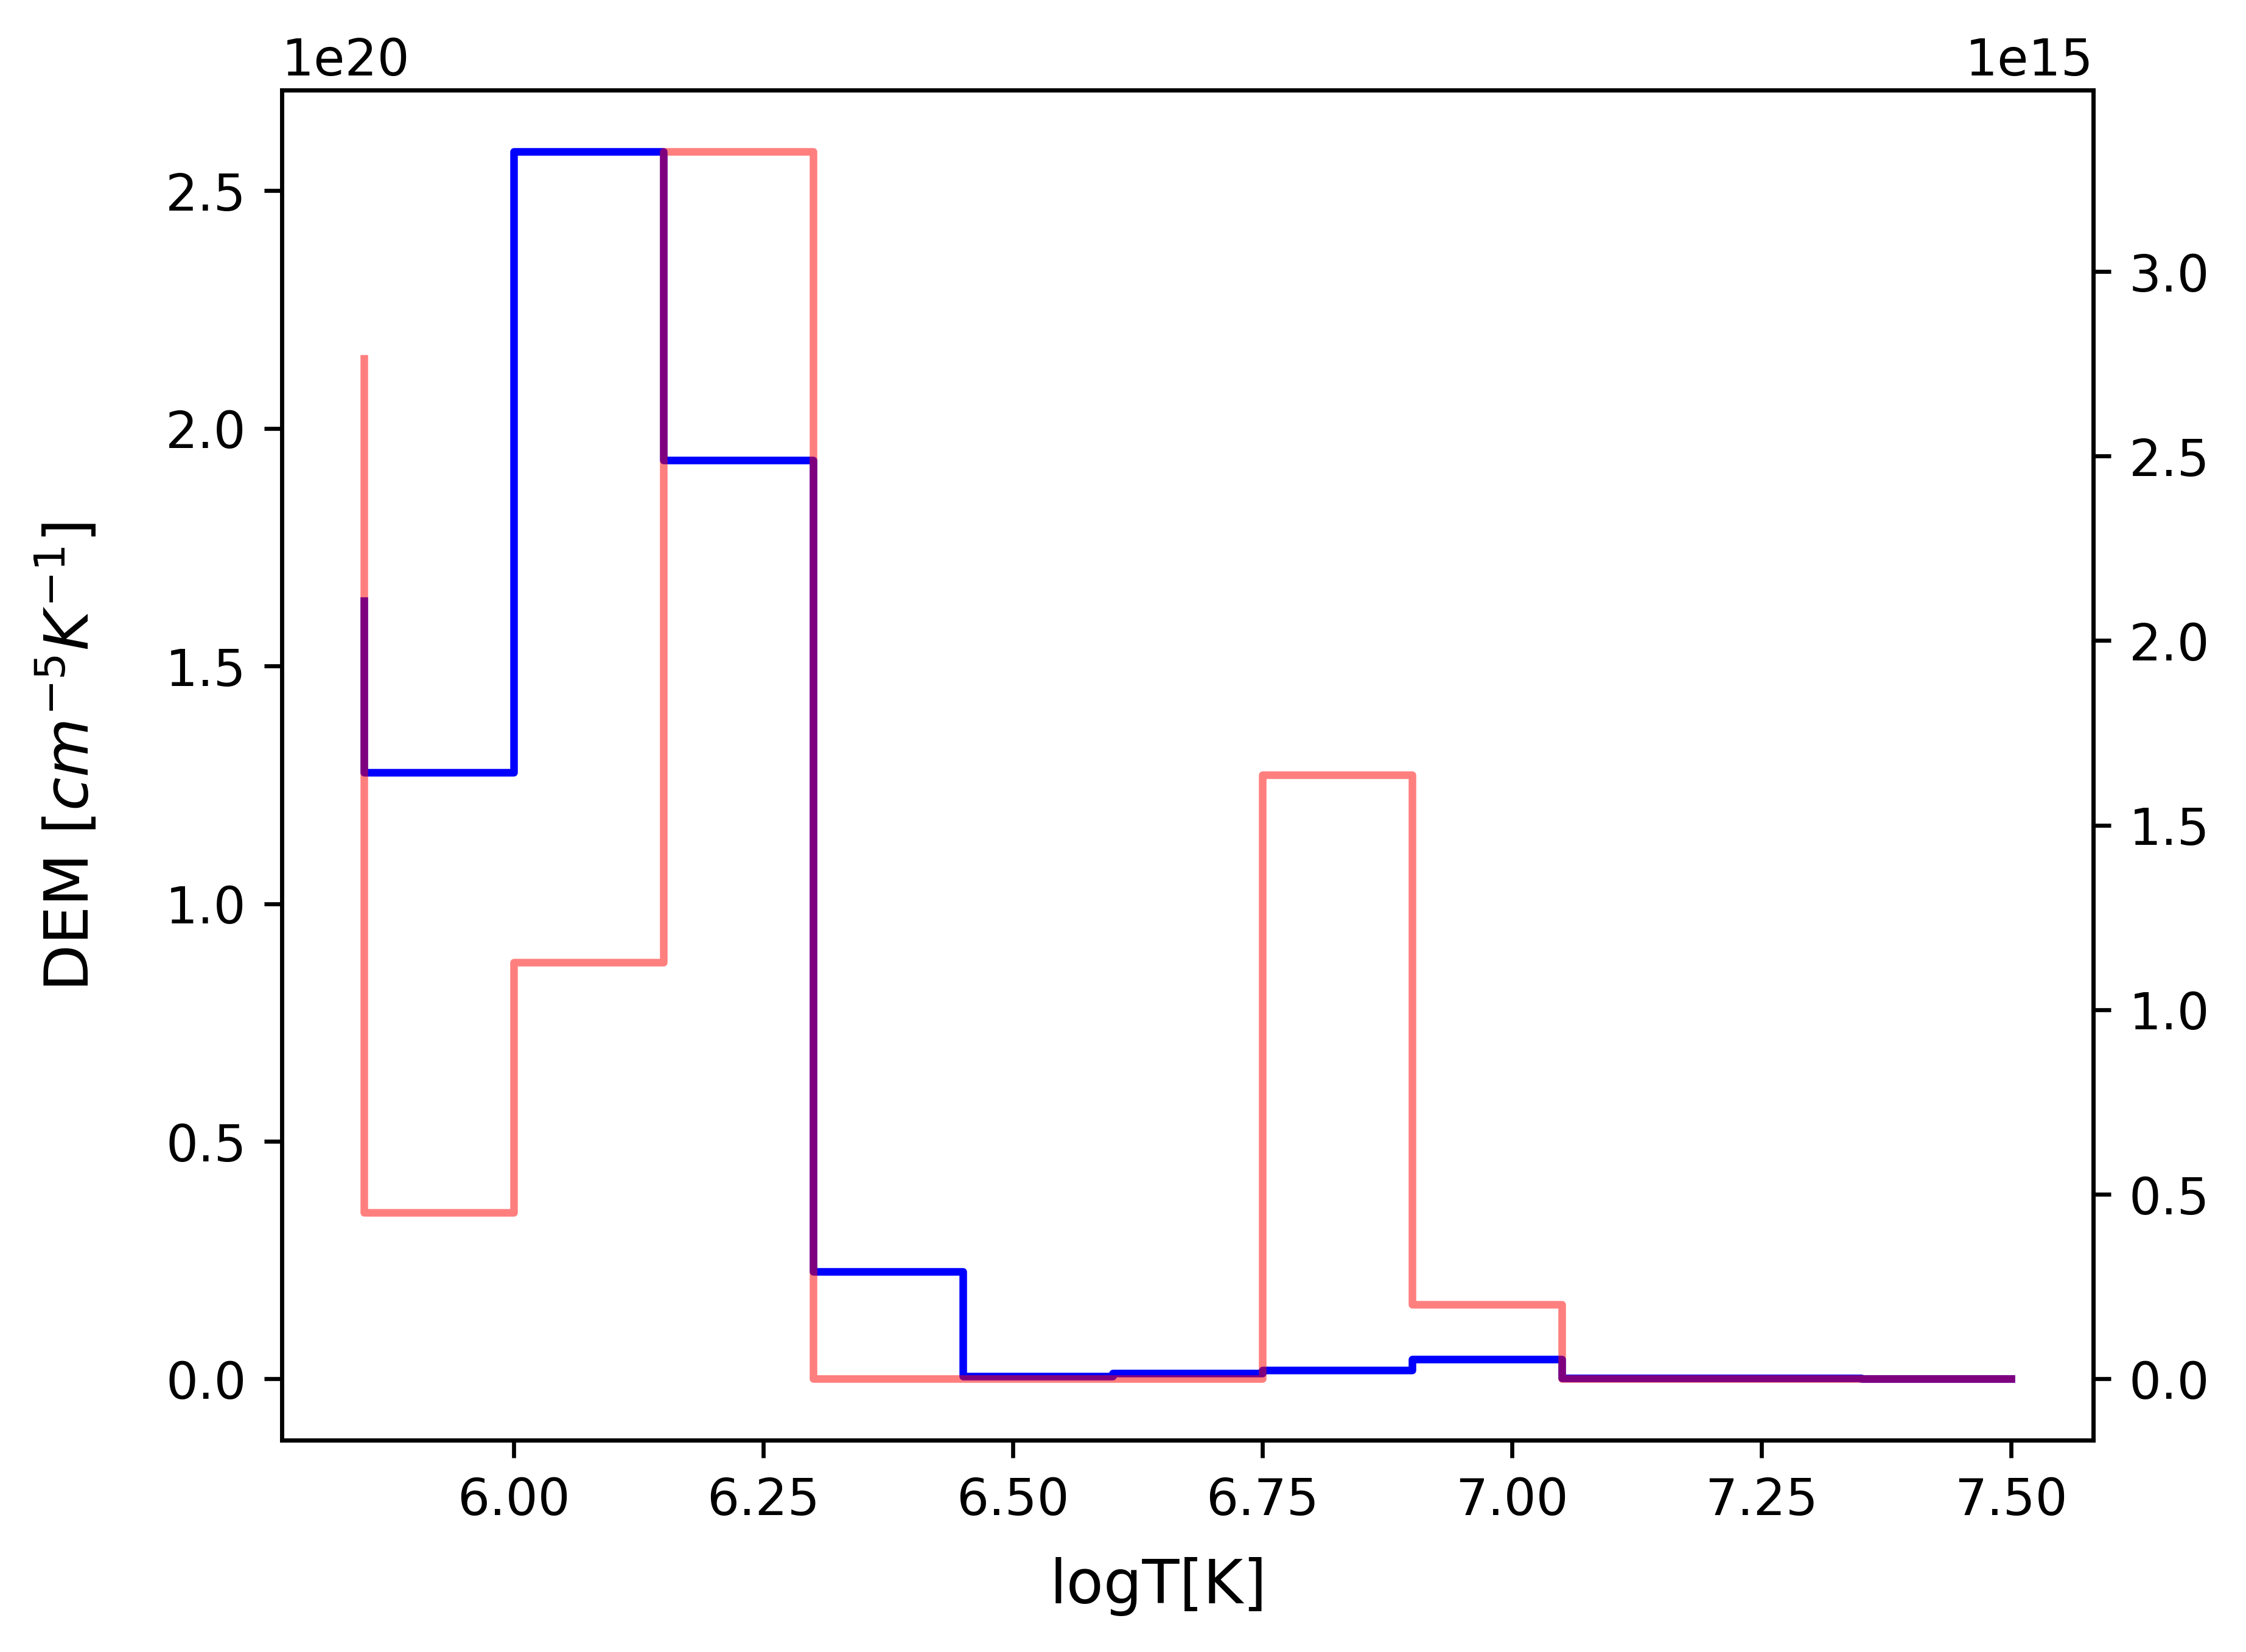
\includegraphics[width=\textwidth]{images/dem_profile_after_event_2011_aug_04.png}
        \caption{After event (10:49 UT)}
    \end{subfigure}

    \caption[DEM profile for \nth{4} August 2011 event]{$DEM$ profile before, during and after the flaring event of \nth{4} August 2011. The red and blue curves correspond to point source and full disk source respectively. $DEM_{ps}$ represents the DEM of the point source.}
    \label{fig:dem_pro_aug_04_2011}
\end{figure}

\begin{figure}[h!]

    \begin{subfigure}[b]{0.3\textwidth}
        \centering
        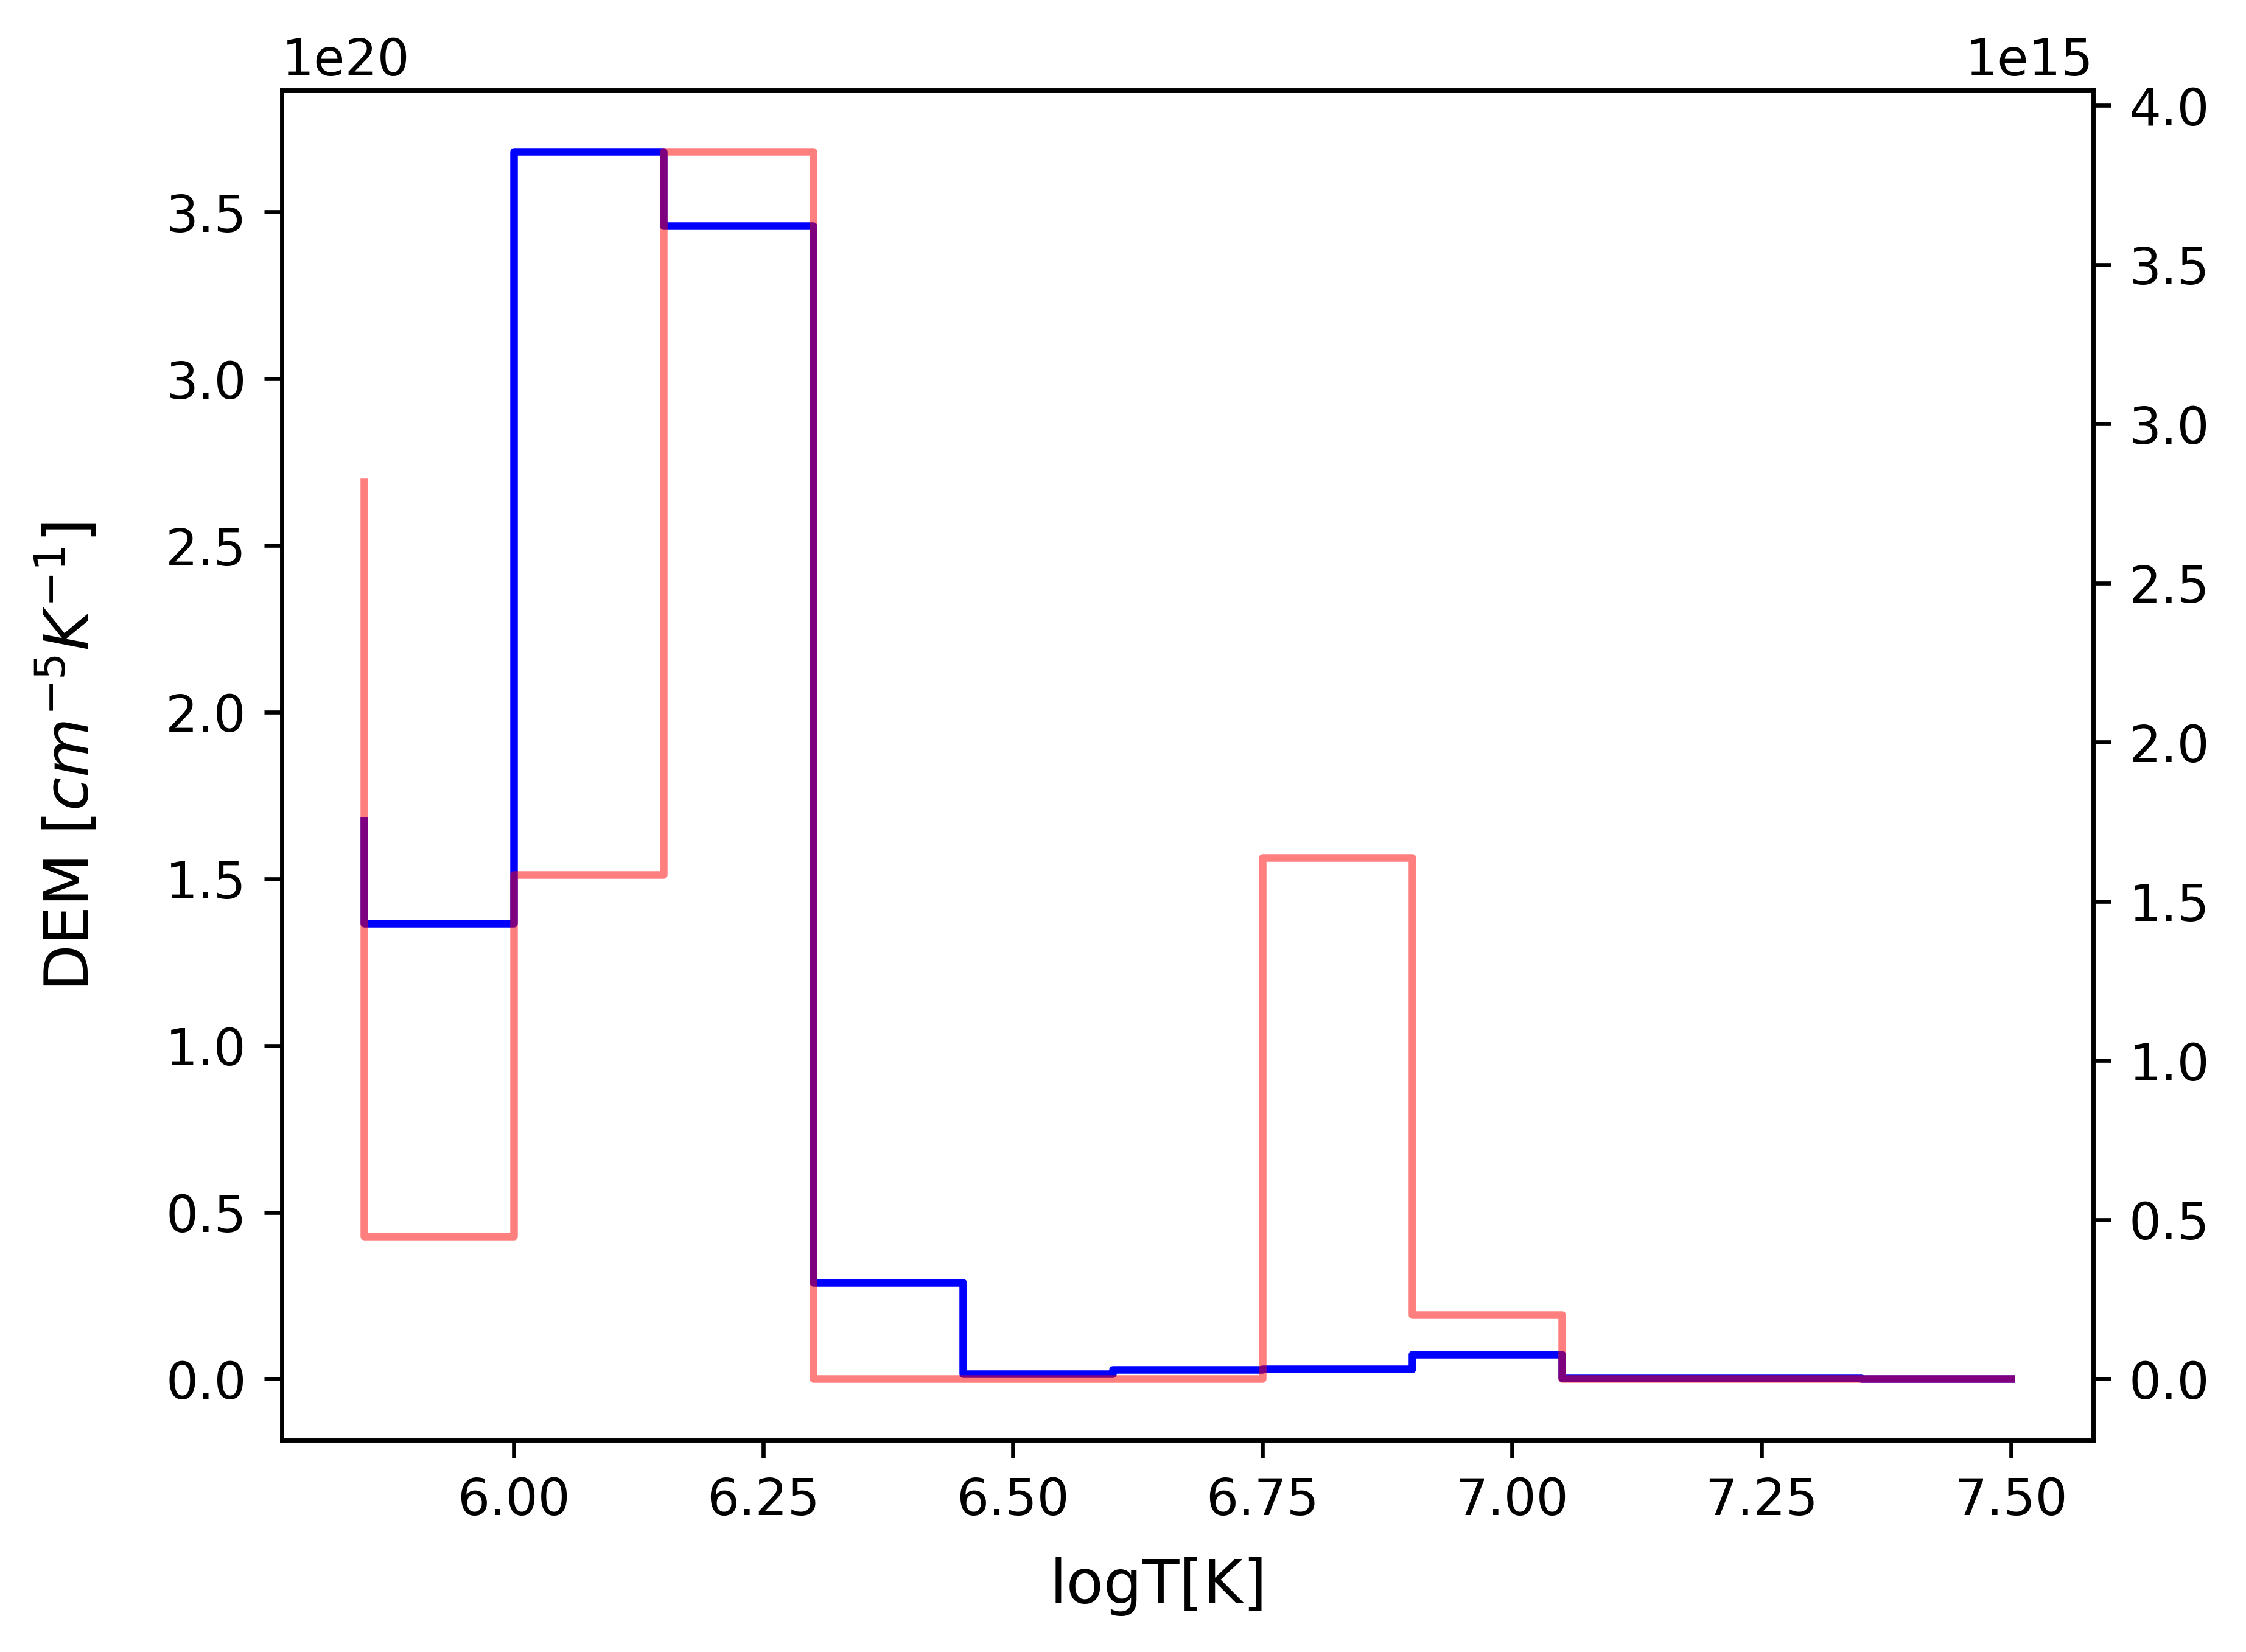
\includegraphics[width=\textwidth]{images/dem_profile_before_event_2012_aug_31.png}
        \caption{Before event (17:19 UT)}
    \end{subfigure}
    \hfill
    \begin{subfigure}[b]{0.3\textwidth}
        \centering
        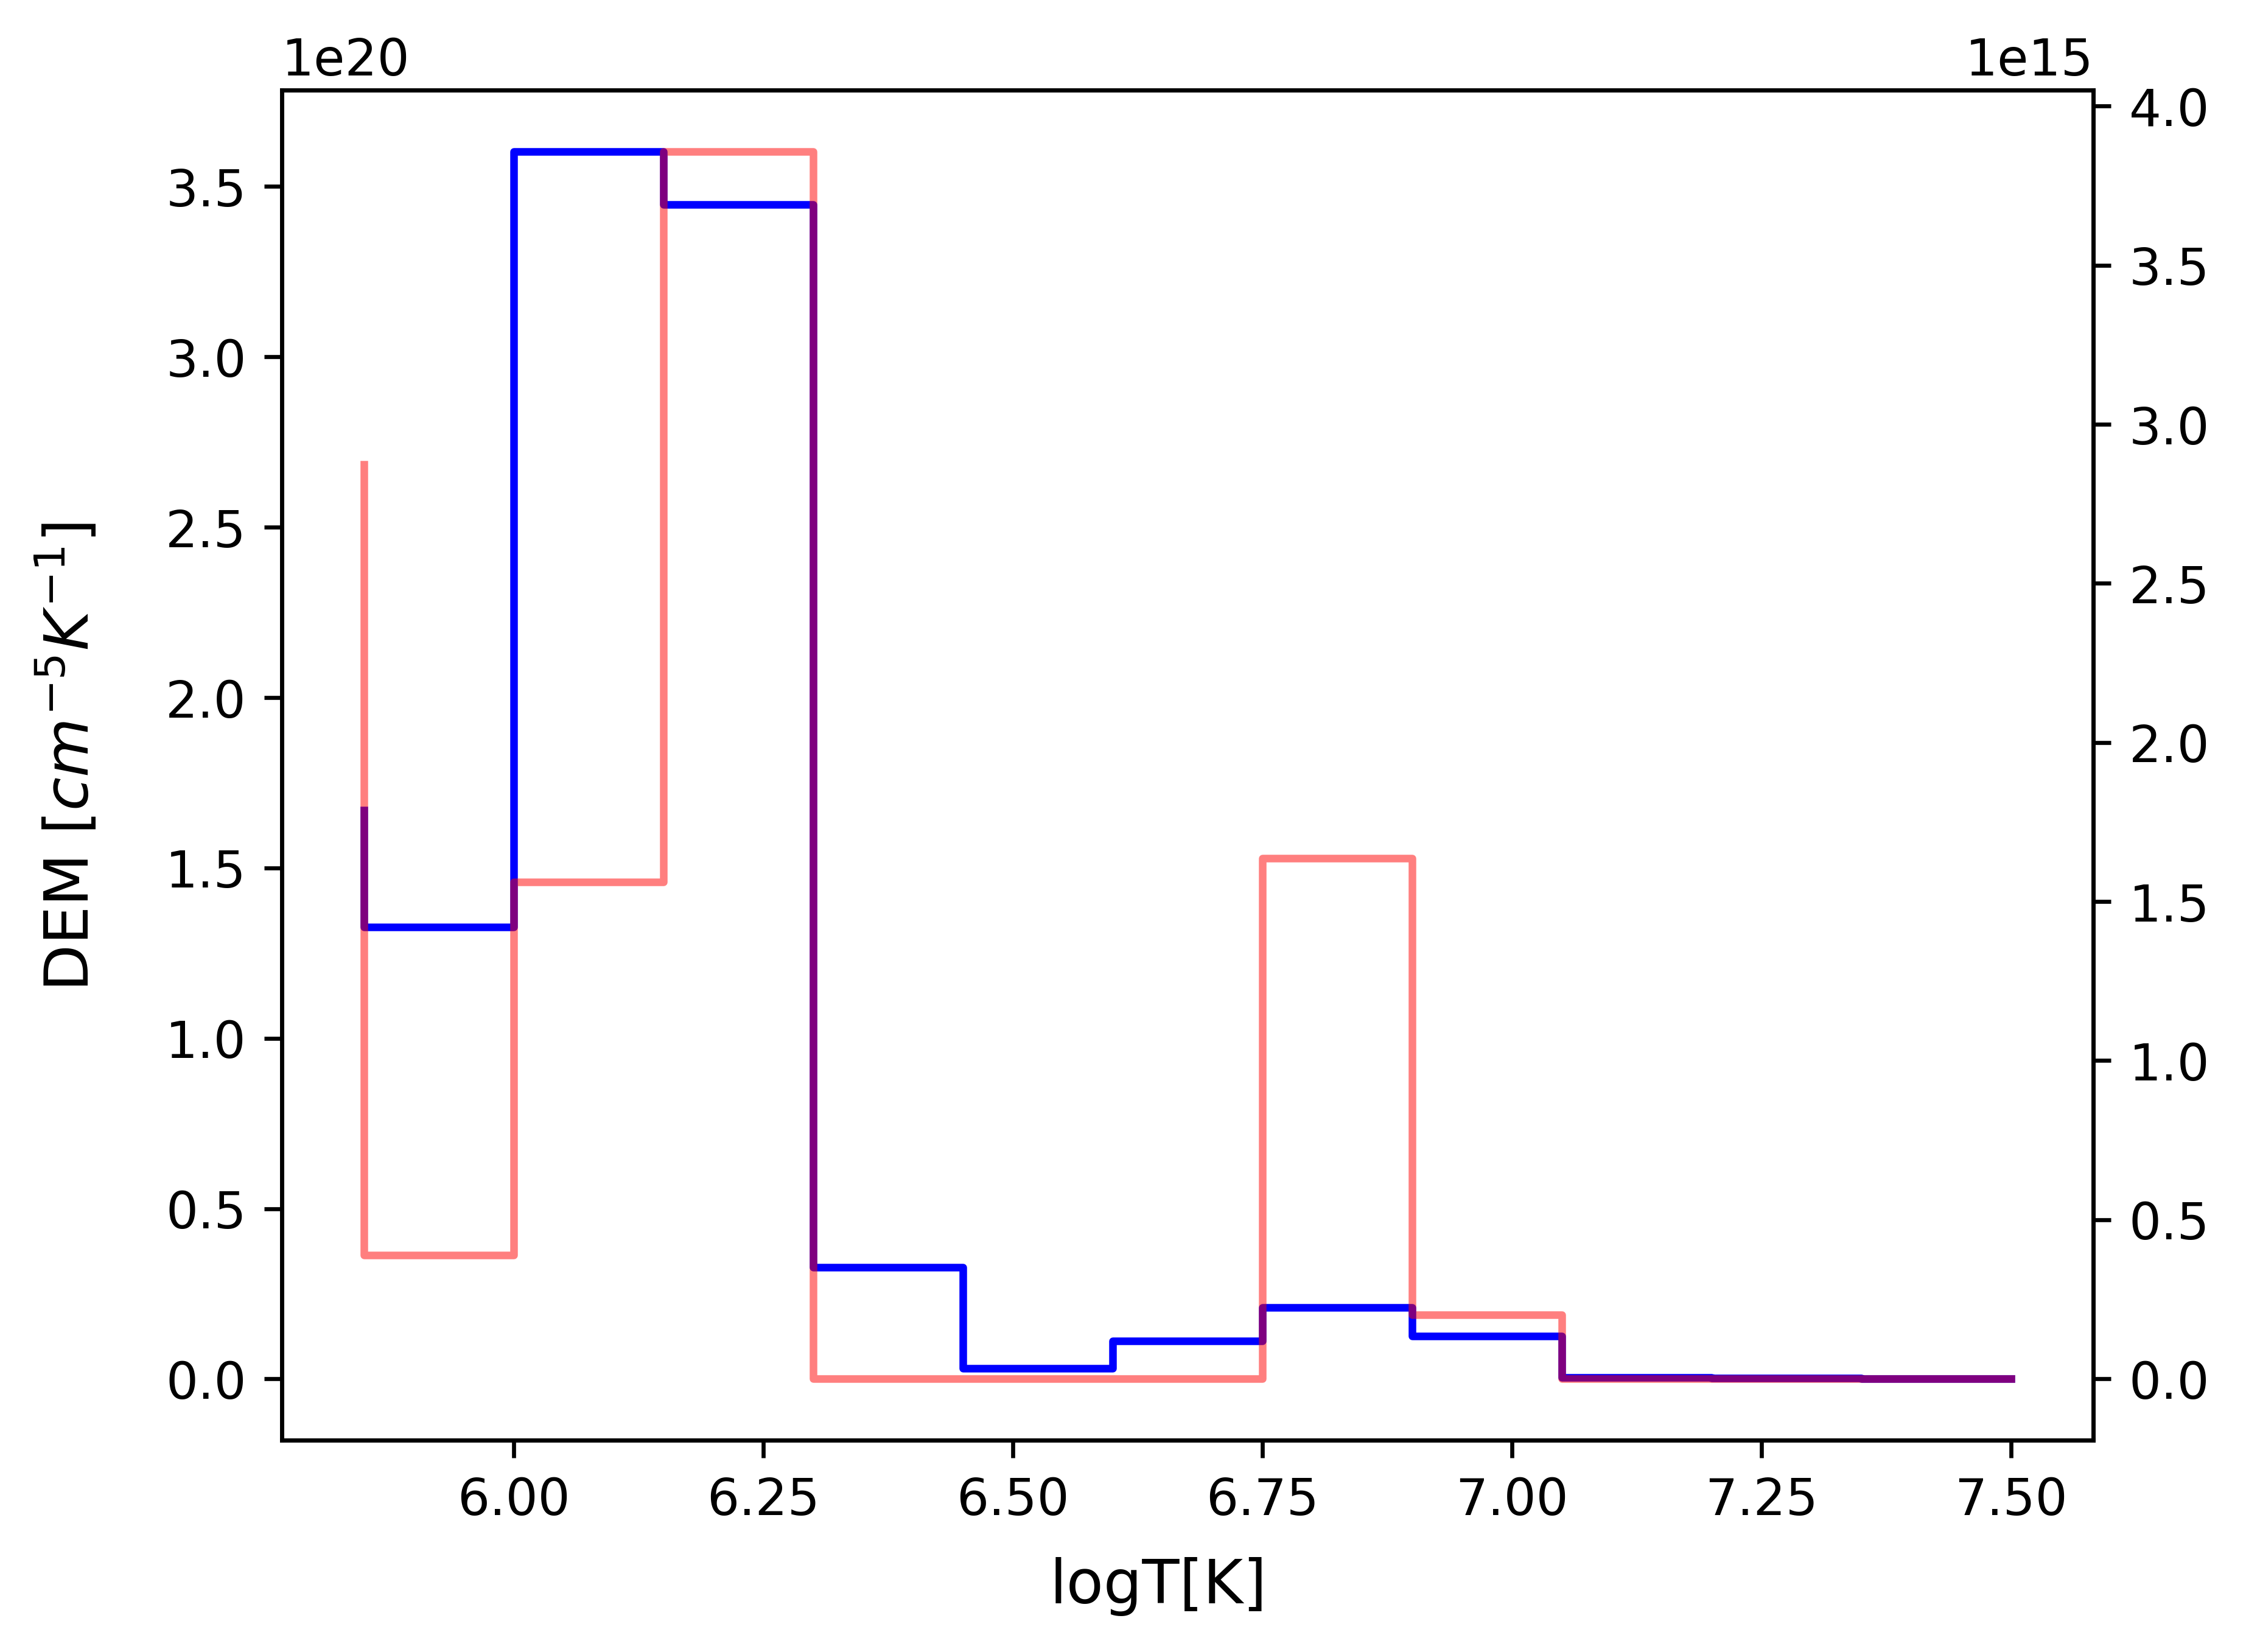
\includegraphics[width=\textwidth]{images/dem_profile_during_event_2012_aug_31.png}
        \caption{During event (20:35 UT)}
        \label{fig:dem_pro_aug_31_2012_b}
    \end{subfigure}
    \hfill
    \begin{subfigure}[b]{0.3\textwidth}
        \centering
        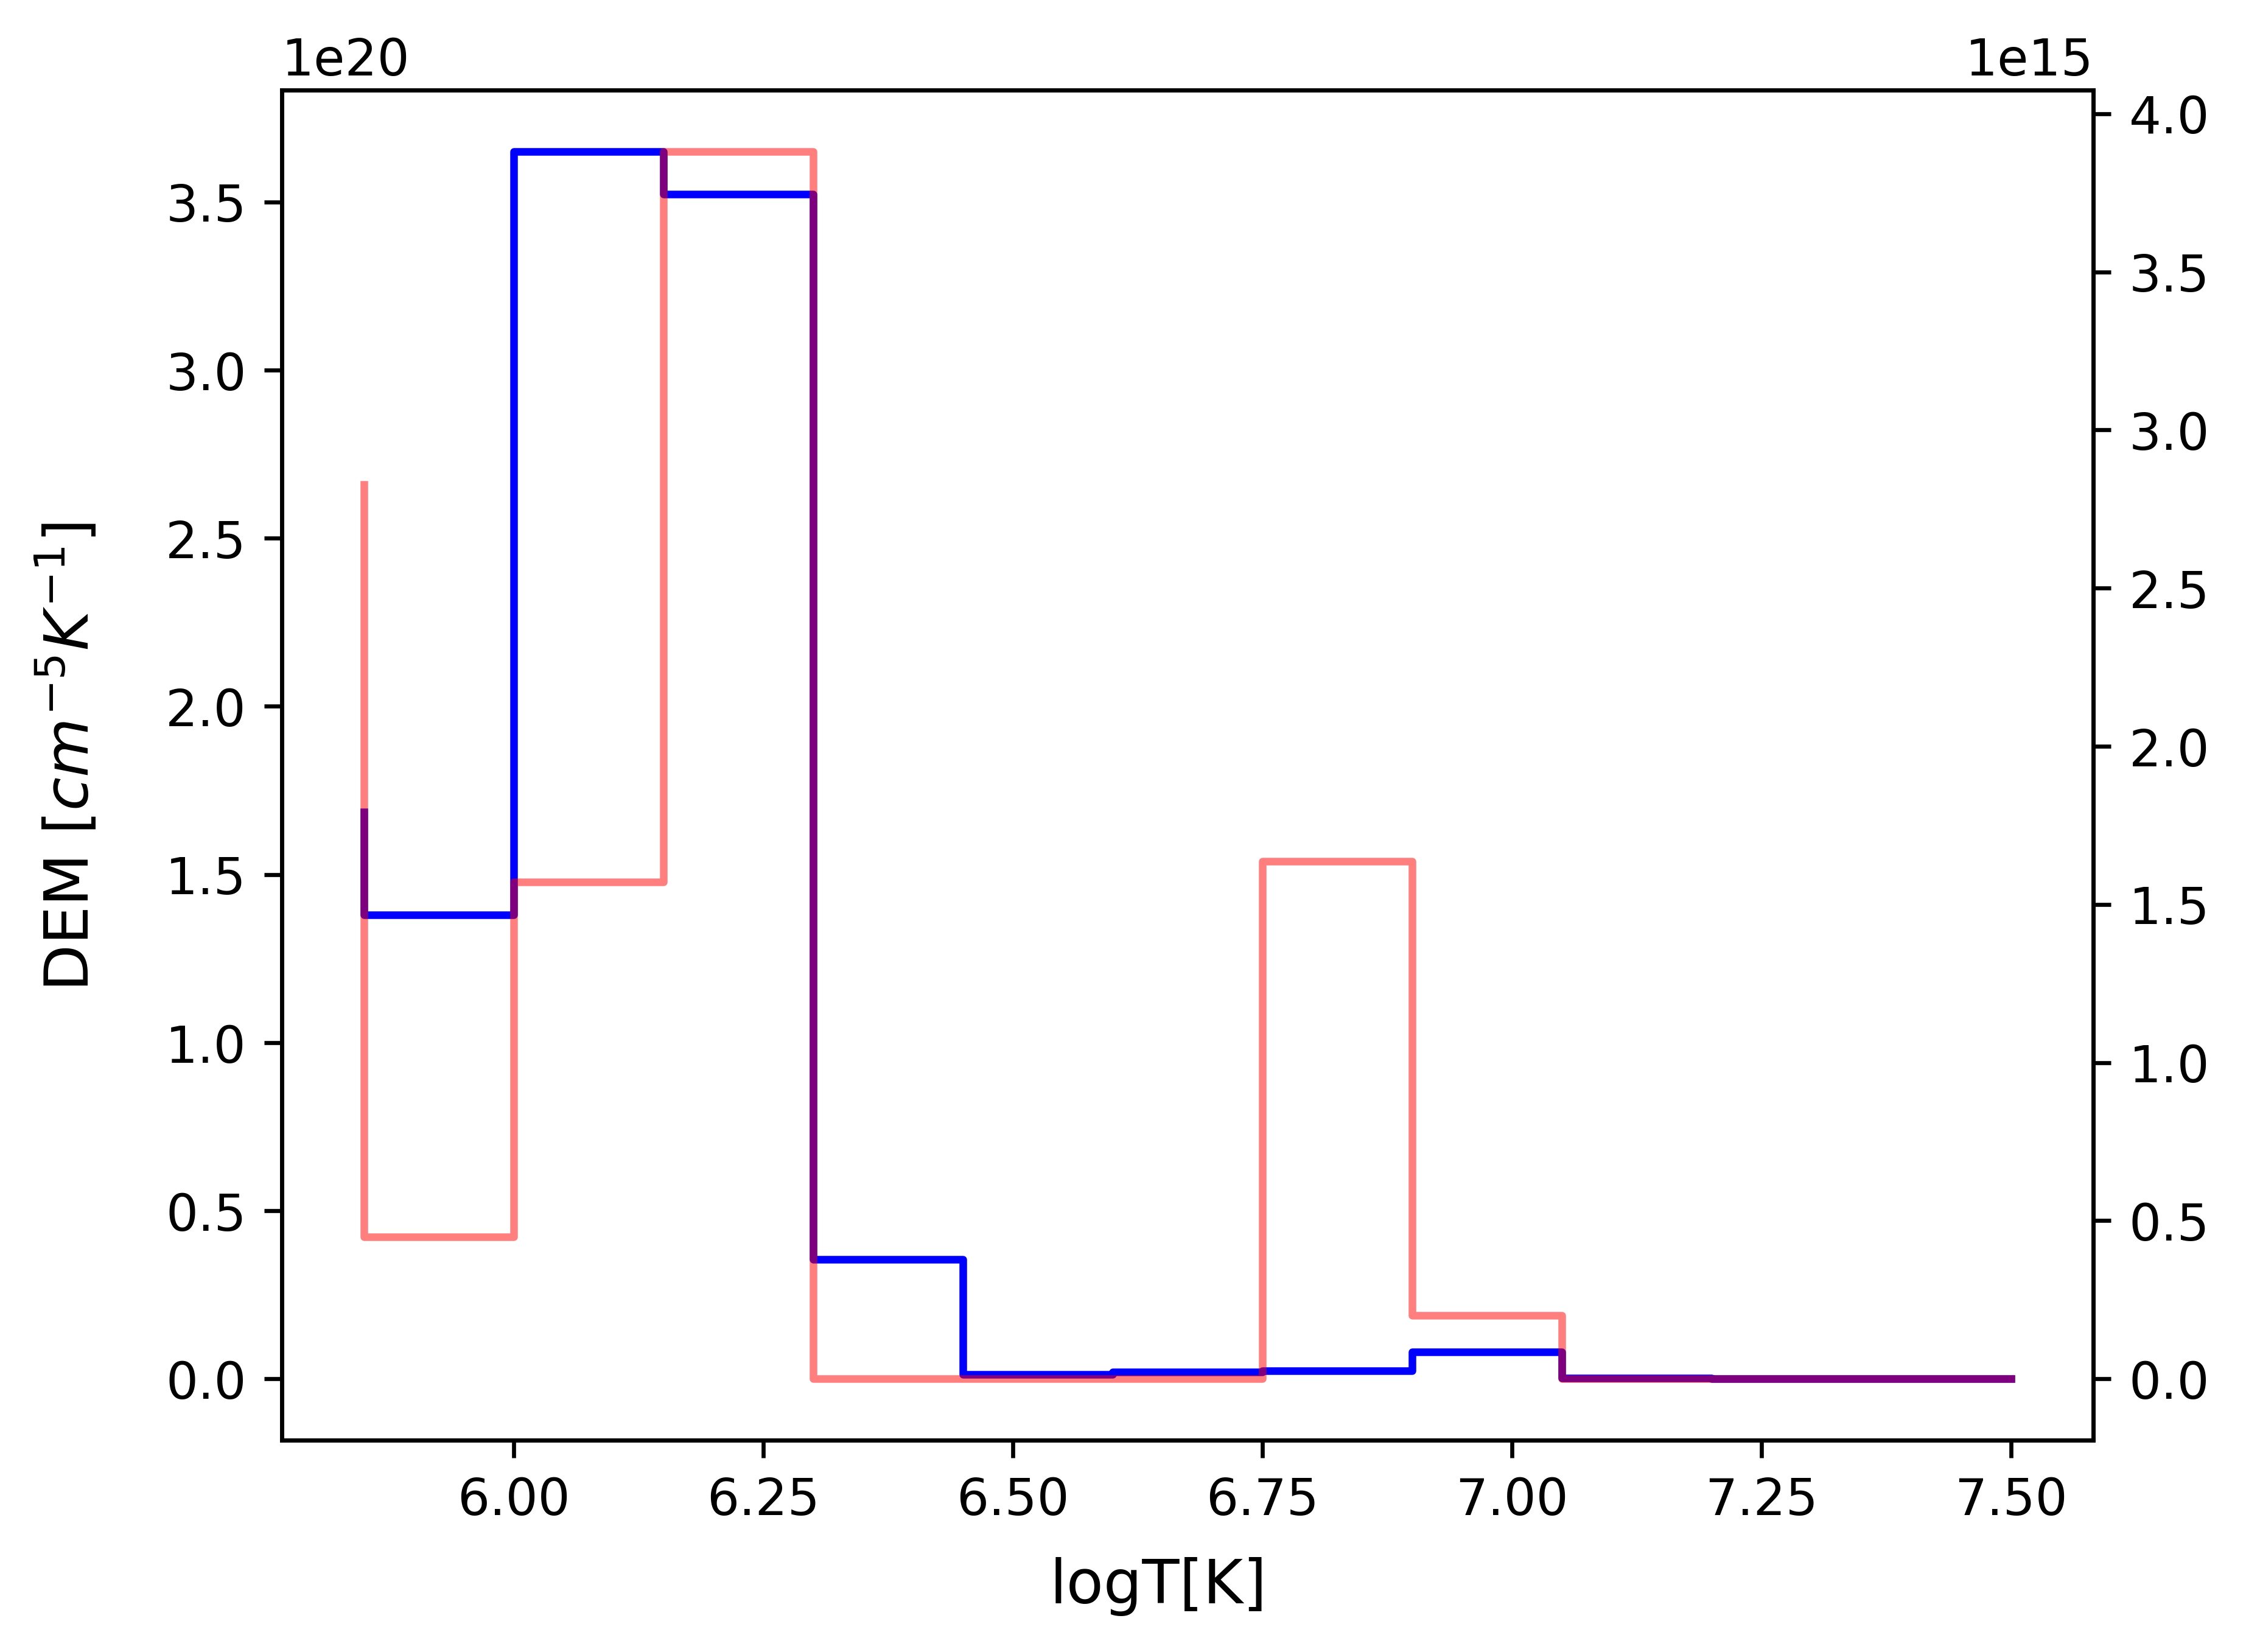
\includegraphics[width=\textwidth]{images/dem_profile_after_event_2012_aug_31.png}
        \caption{After event (\nth{1} Sep 2011 03:57 UT)}
    \end{subfigure}

    \caption[DEM profile for \nth{31} August 2012 Event]{$DEM$ profile before, during and after the flaring event of \nth{31} August 2012.}
    \label{fig:dem_pro_aug_31_2012}
\end{figure}

\begin{figure}[h!]

    \begin{subfigure}[b]{0.3\textwidth}
        \centering
        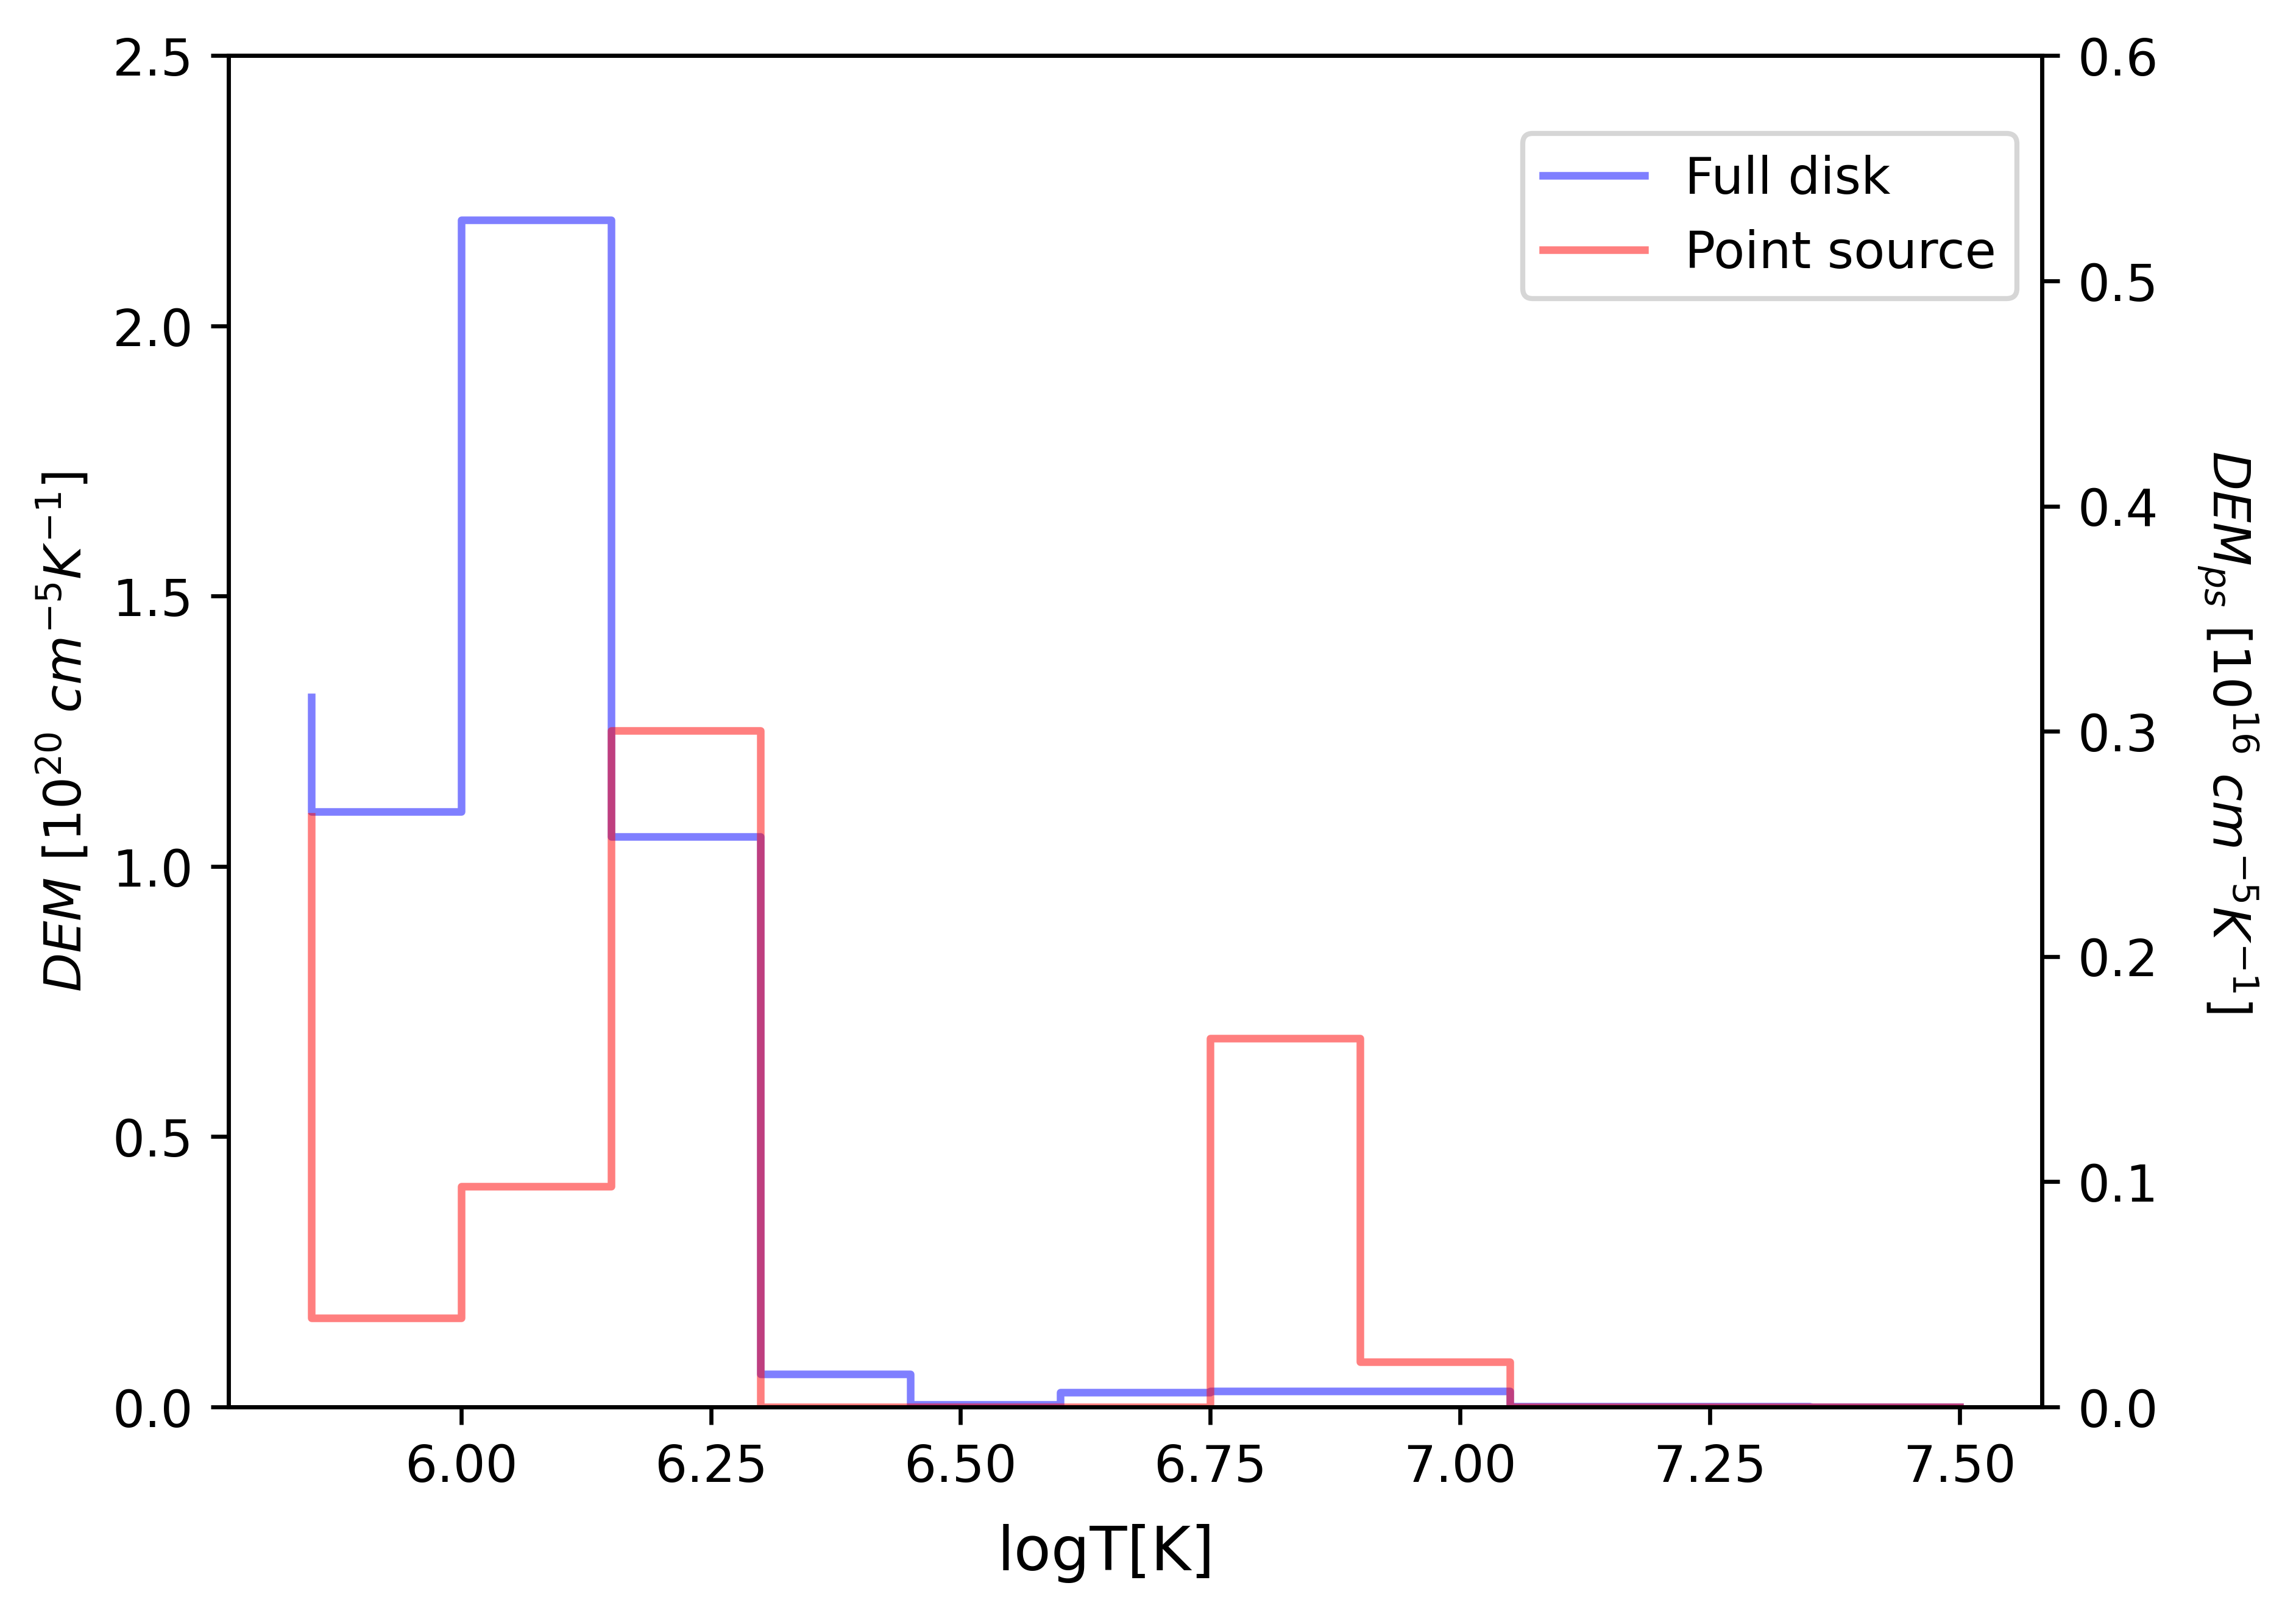
\includegraphics[width=\textwidth]{images/dem_profile_before_event_2021_oct_28.png}
        \caption{Before event (13:23 UT)}
    \end{subfigure}
    \hfill
    \begin{subfigure}[b]{0.3\textwidth}
        \centering
        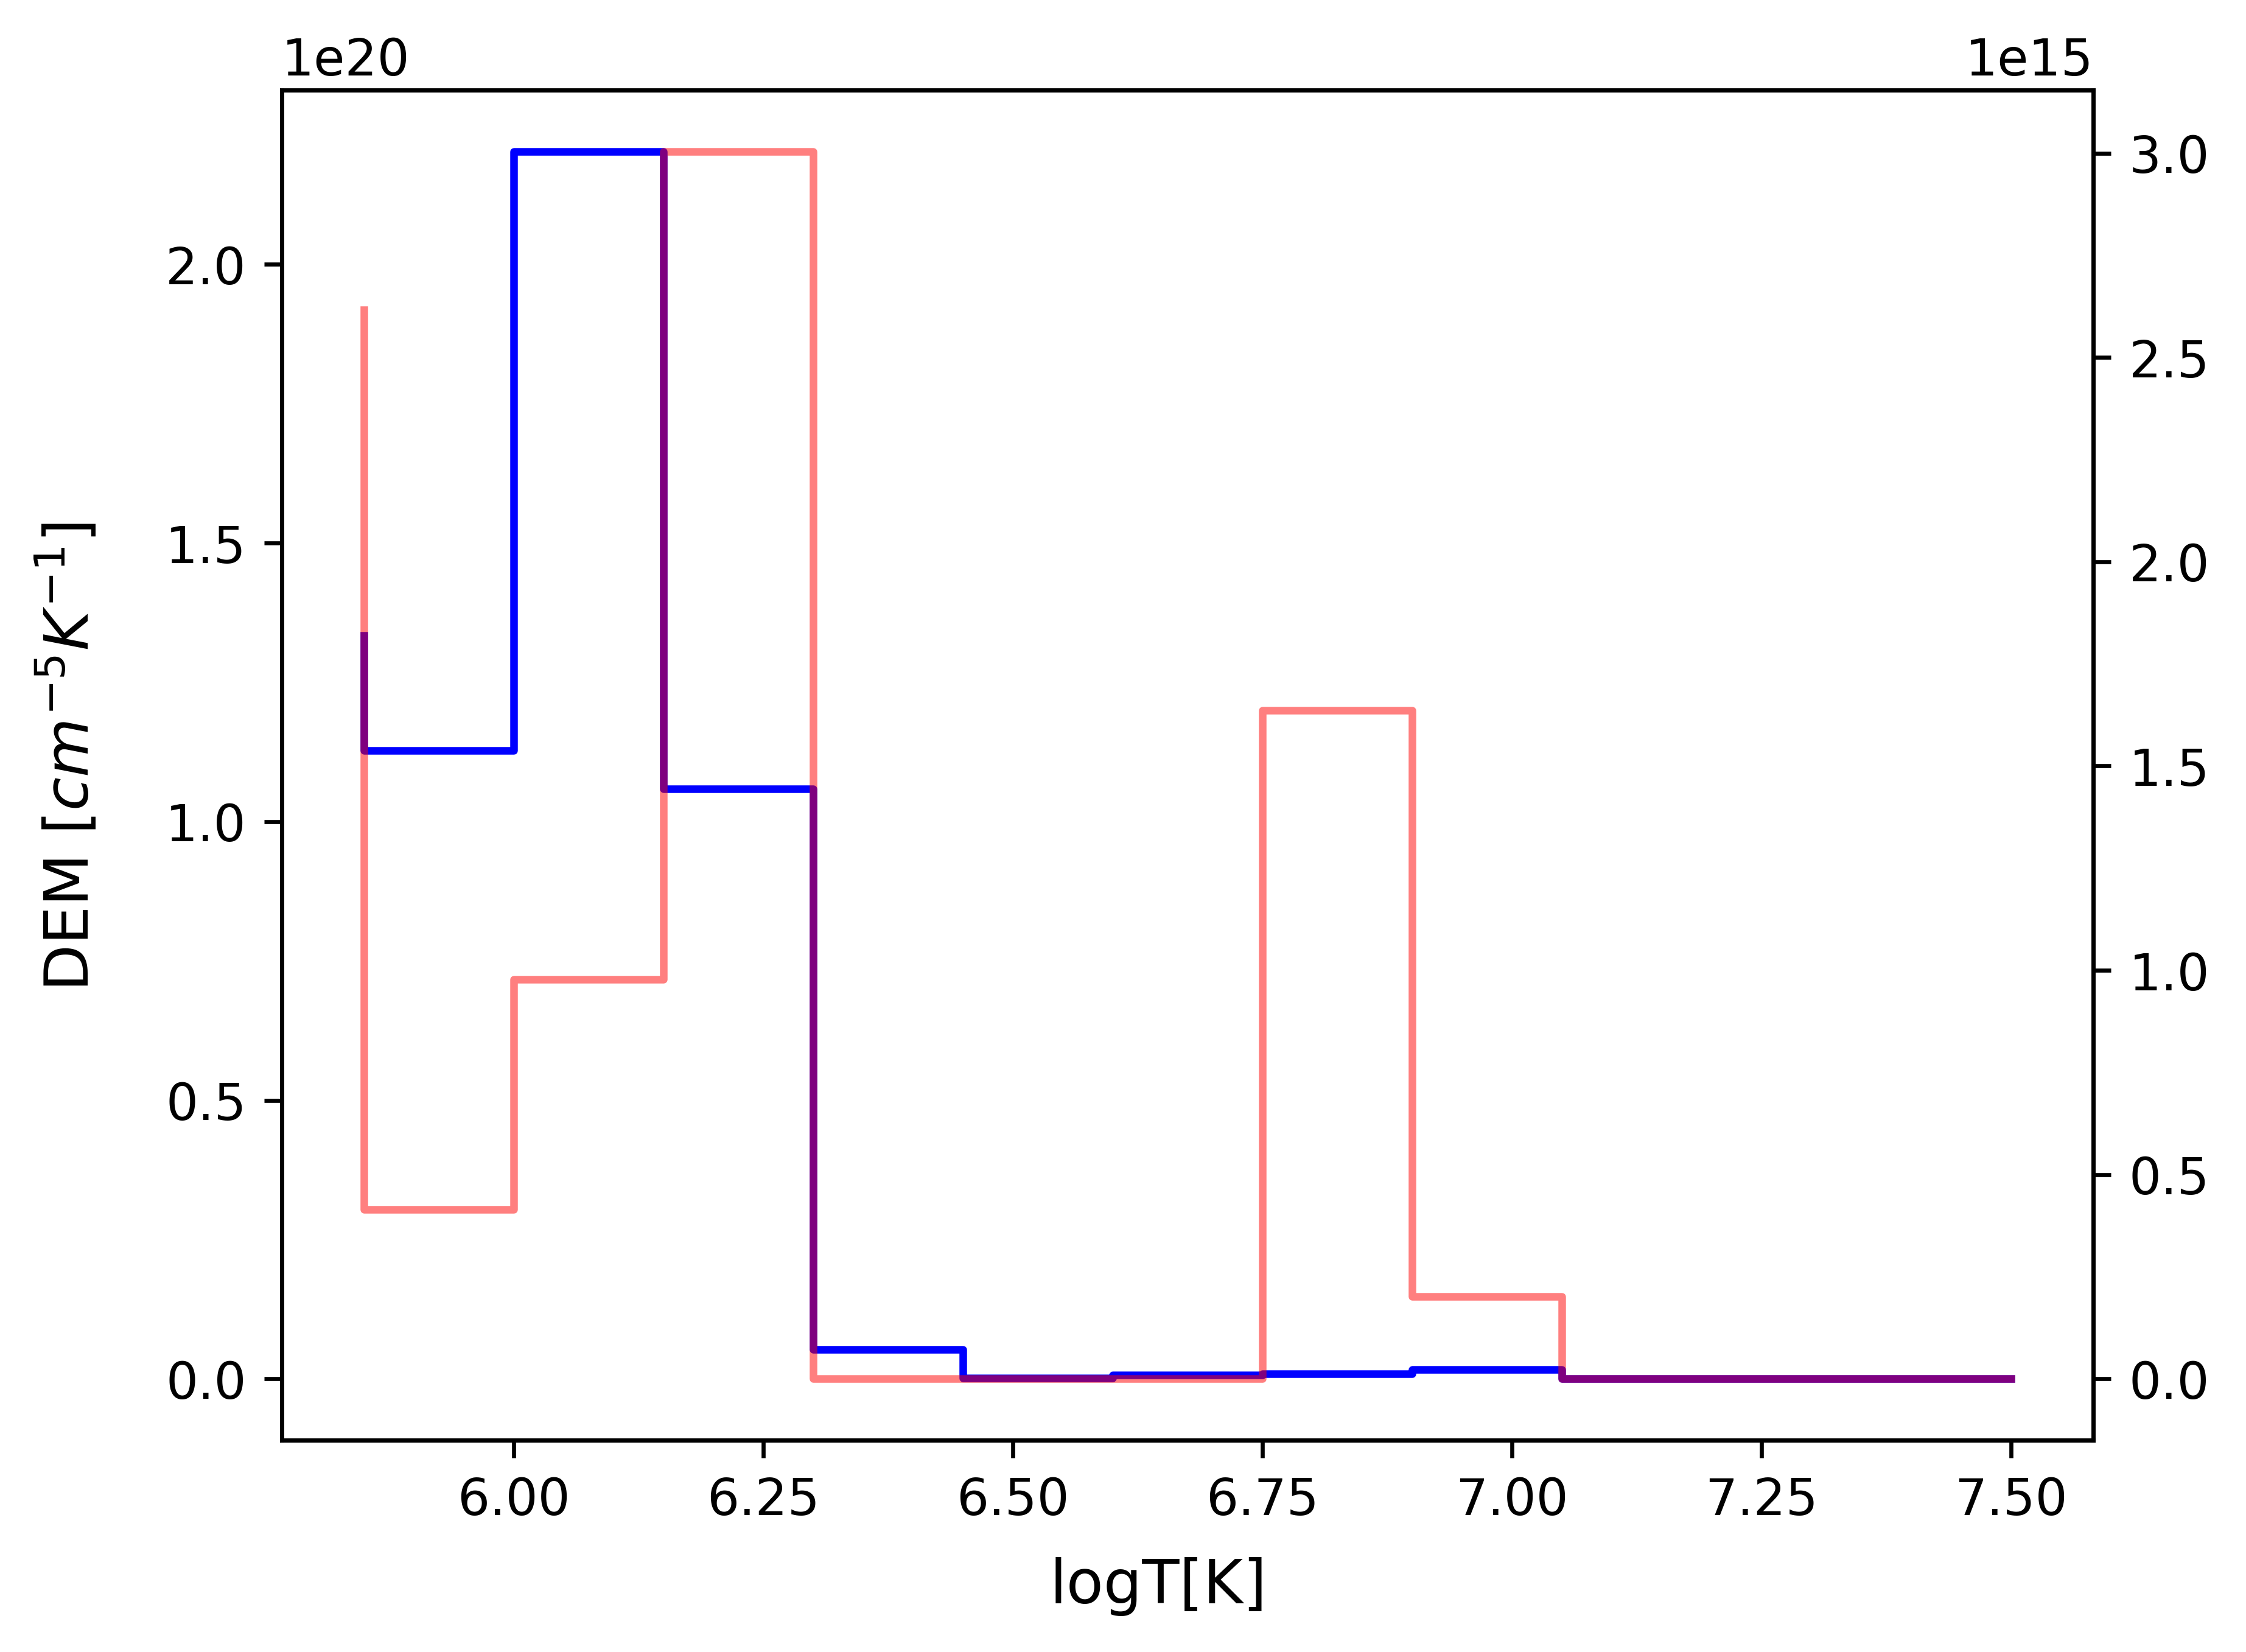
\includegraphics[width=\textwidth]{images/dem_profile_during_event_2021_oct_28.png}
        \caption{During event (15:35 UT)}
    \end{subfigure}
    \hfill
    \begin{subfigure}[b]{0.3\textwidth}
        \centering
        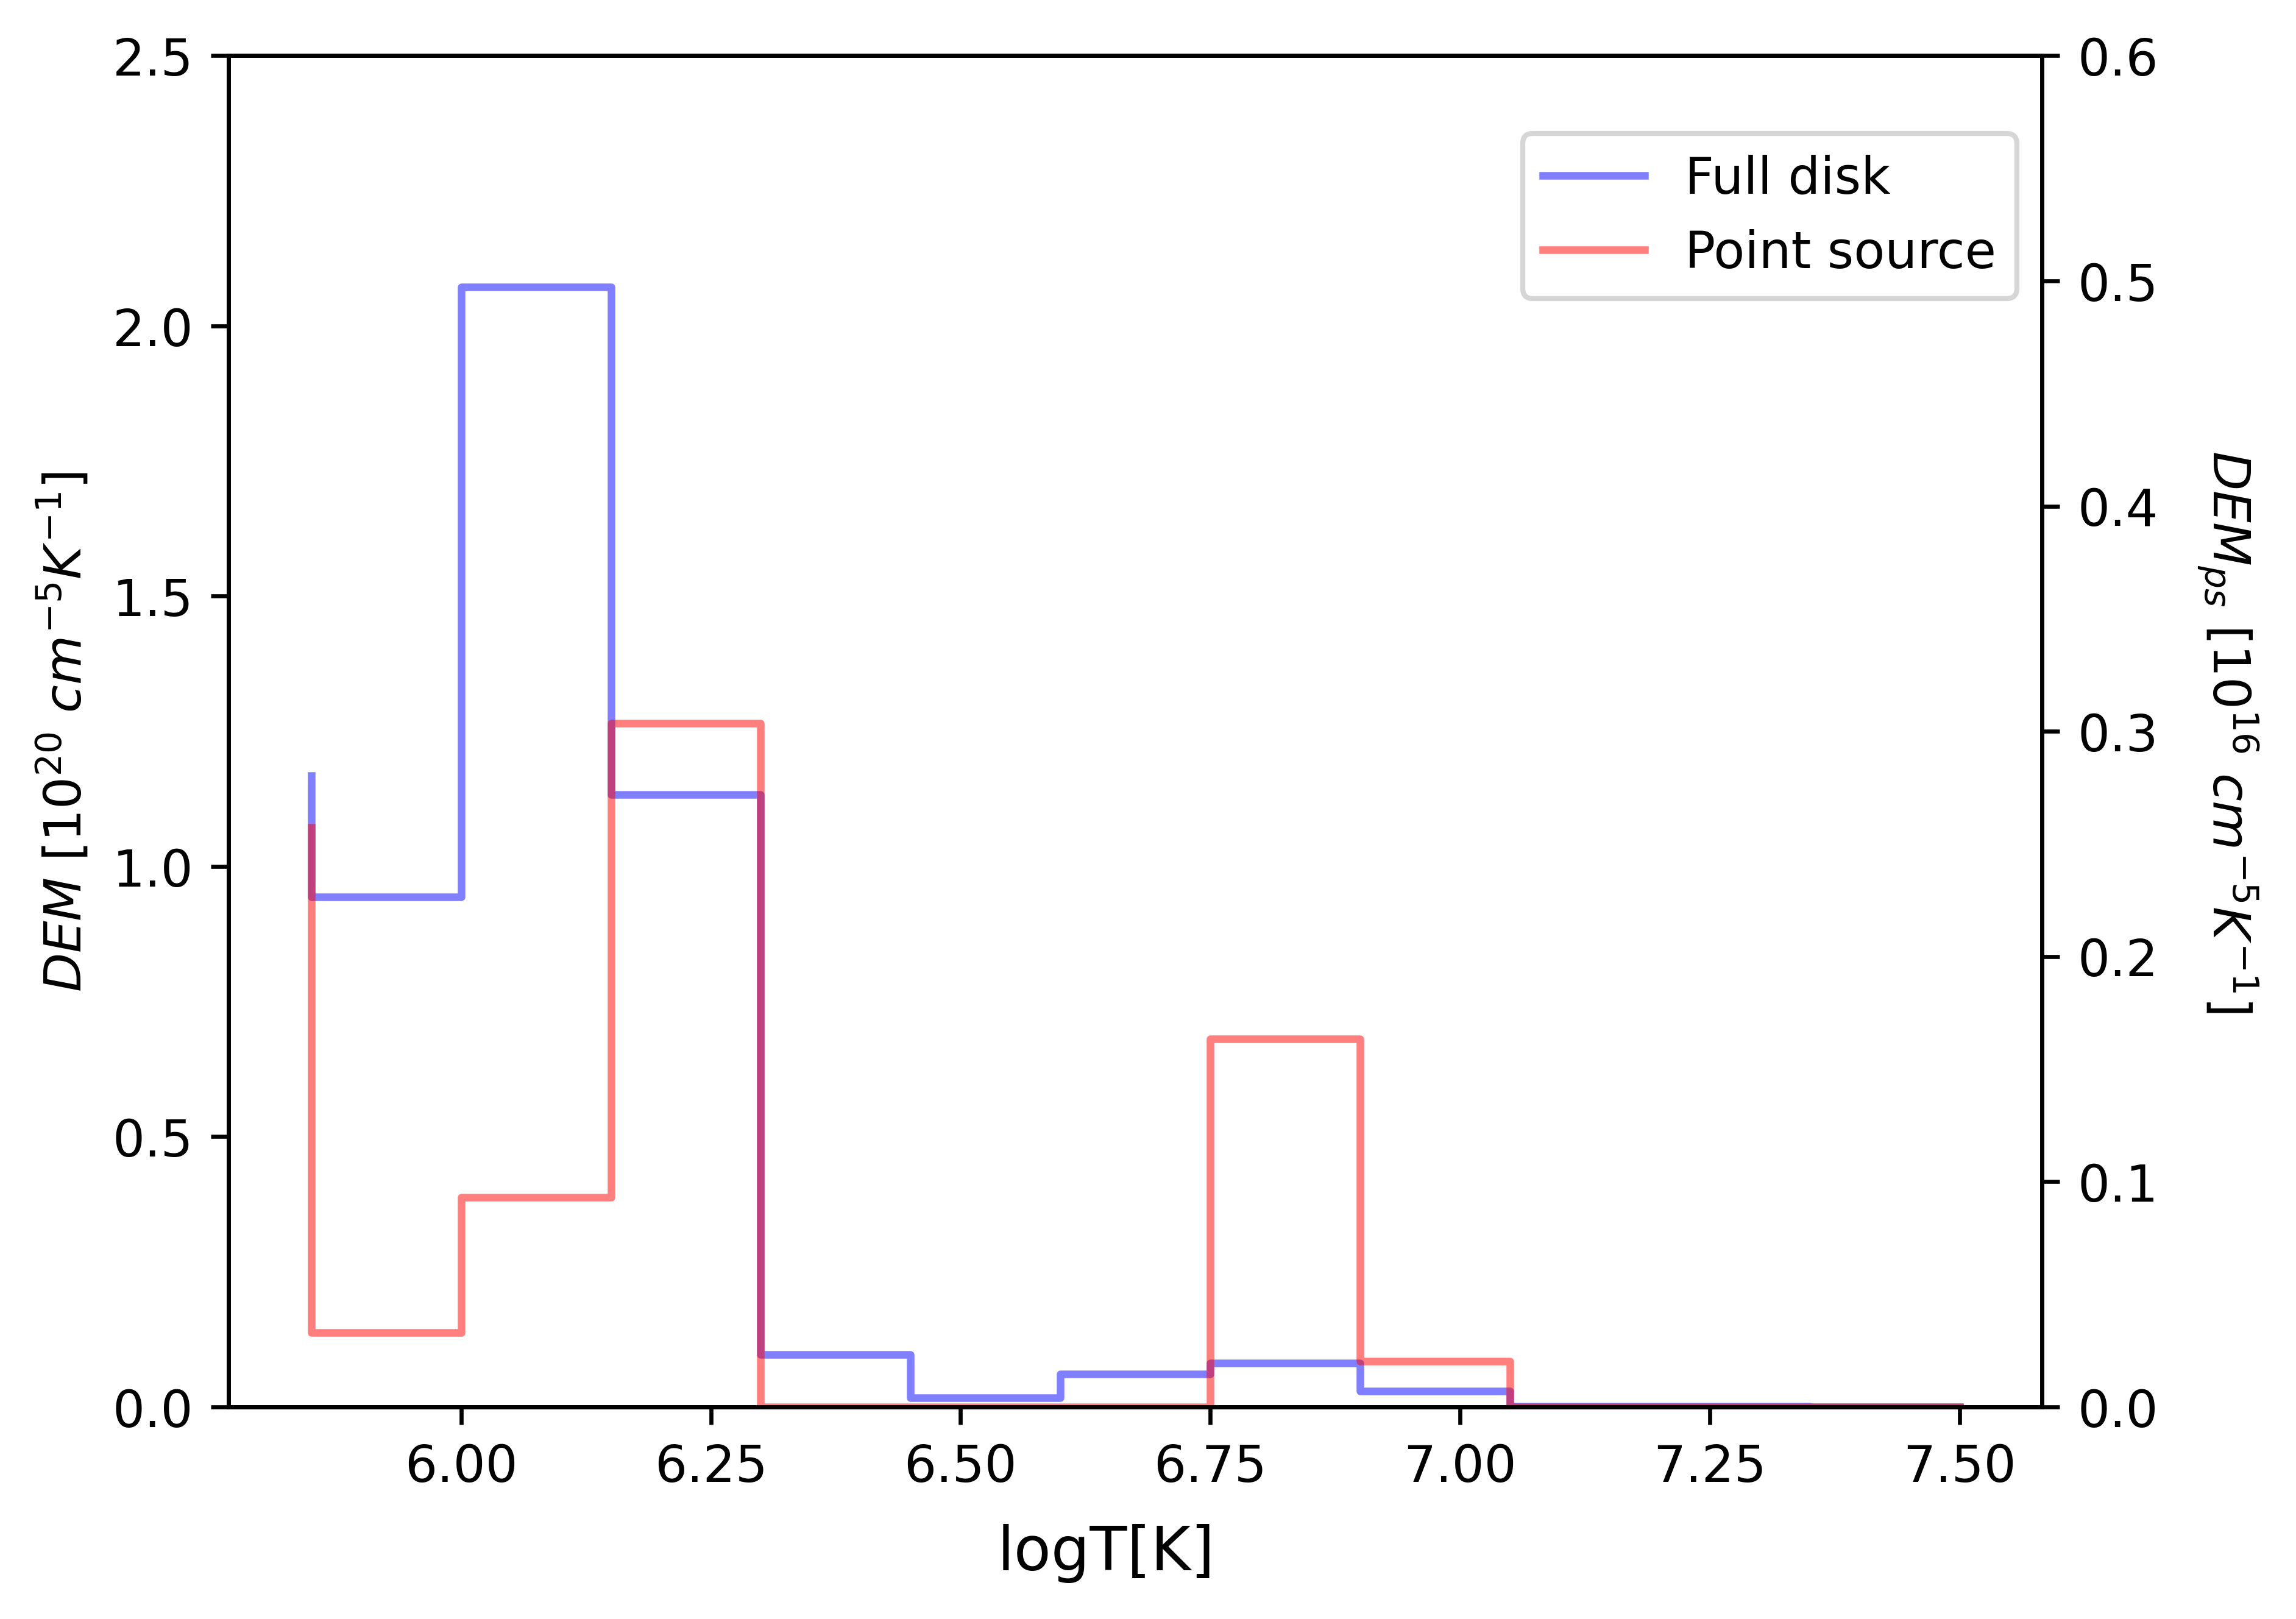
\includegraphics[width=\textwidth]{images/dem_profile_after_event_2021_oct_28.png}
        \caption{After event (17:29 UT)}
    \end{subfigure}
    \caption[DEM profile for \nth{28} October 2021 event]{$DEM$ profile before, during and after the flaring event of \nth{28} October 2021.}
    \label{fig:dem_pro_oct_28_2021}
\end{figure}

The temperature distribution of the plasma at different sections of an event can be studied through it's DEM profile (DEM profile is a plot of logT vs DEM). The DEM profiles before, during and after the event has been shown in \cref{fig:dem_pro_aug_04_2011}, \cref{fig:dem_pro_aug_31_2012} and \cref{fig:dem_pro_oct_28_2021} for the events of \nth{4} August 2011, \nth{31} August 2012 and \nth{28} October 2021 respectively.

In \cref{fig:dem_pro_aug_04_2011} and \cref{fig:dem_pro_aug_31_2012} the DEM profile (full disk + point source) before and after the event looks similar. \Cref{fig:dem_pro_aug_04_2011_b} shows the increase in full disk emission during the event in the range logT $\sim$ [6.5, 7.0] and point source emission increases in the range logT $\sim$ [6.125, 6.25]. \Cref{fig:dem_pro_aug_31_2012_b} shows a slight increase in the full disk emission in the range logT $\sim$ [6.6, 7.0], but not change in the point source DEM is observed.

\Cref{fig:dem_pro_oct_28_2021} shows increase in emission of full disk in the range logT $\sim$ [6.25, 7.25] during the event. But, there is slight increase in the emission in this range after the event (compared to before the event), which is not observed in the previous two events.

\section{Discussion and Conclusion}

In this study, we have presented a comprehensive analysis of CMEs on the Sun through DEM analysis, incorporating innovative methodologies and novel approaches. We have analyzed three CME events, each associated with unique solar phenomena like coronal dimming, filament eruption and ground level enhancement CME event. Our DEM analysis shows that the maximum dimming depth temperature range for the event of \nth{4} August 2011 has been seen in the range logT = [5.85, 6.15], shedding light into the underlying physical mechanisms driving dimming phenomena. We demonstrated the process of converting full disk image to a point source, to study the Sun-star CME relation. The correlation between the full disk and point source DEM is high in the temperature range below logT $\sim$ 6.45. Discrepancy in the value of DEM is observed between the point source and the full disk which might be because of many reasons like naively averaging the entire image when reducing to a point source, error in the DEM inversion.\\

The pointification of the full disk image has rooms for improvement, which has to be taken care of during further studies. Approach like naively directly averaging the pixel values of images and reduction to point source poses problems at places where the corresponding DEM solutions either do not exist or is very minute in the full disk image, leading to incorrect averaging of pixels for the case of point source. Hence, careful reduction to point source is necessary. Moving forward, we plan to improve the point source reduction process, increase the temperature interval to increase the accuracy of the DEM solutions and look at more events, so that we can do a statistical analysis, which would enable us to check if the correlations observed actually hold for a larger set of events. Additionally, we also would look at CME events originating at different regions on the Sun and understand it's effect on the coronal dimming and temperature variations of the Solar corona.

%%% Local Variables:
%%% mode: LaTeX
%%% TeX-master: "main"
%%% End:
